\chapter{Interakcija svetlobe s snovjo}

V prejšnjih poglavjih smo obravnavali svetlobo v praznem prostoru. Oglejmo si
zdaj osnovne procese interakcije svetlobe s snovjo. To je seveda zelo
obširna tema in jo bomo obdelali le toliko, kolikor je treba za
obravnavo ojačevanja svetlobe s stimulirano emisijo, ki je osnova za
delovanje laserjev. Najprej bomo na kratko pogledali termodinamsko ravnovesje 
svetlobe v stiku s toplotnim rezervoarjem, torej sevanje črnega telesa, ki 
zahteva kvantno obravnavo elektromagnetnega polja. Nato bomo vpeljali fenomenološki
Einsteinov opis mikroskopskih procesov absorpcije, spontane in stimulirane
emisije in pokazali, da ti procesi niso neodvisni. Izpeljali bomo
izraze za absorpcijski koeficient in koeficient ojačanja, na koncu poglavja
pa bomo nakazali še kvantnomehansko izpeljavo verjetnosti za prehod
atoma iz višjega energijskega stanja v nižje s sevanjem.

\section{Kvantizacija elektromagnetnega polja}

Ravni valovi\index{Ravni val} so enostavne in zelo prikladne rešitve valovne 
enačbe~(\ref{eq:valovna-skalarna}), zato jih pri reševanju problemov pogosto uporabimo kot 
bazo, po kateri razvijemo elektromagnetno polje\index{Elektromagnetno valovanje}. Možen je razvoj
po celotnem prostoru, vendar je tedaj nekoliko nerodna normalizacija baznih
funkcij. Če se omejimo na le del prostora, se temu problemu izognemo. Mora pa biti 
izbrani del prostora dovolj velik, da končni rezultat ni odvisen od izbire 
njegove velikosti in oblike.

Najpreprosteje je vzeti votlino v obliki velike kocke s stranico
$L$ in idealno prevodnimi stenami. Rešitve Maxwellovih enačb~(\ref{eq:Maxwell1} do \ref{eq:Maxwell4}) 
znotraj take votline so ob upoštevanju robnih pogojev (enačba~\ref{eq:robni-pogoji}) 
stoječa valovanja. Zapišemo jih v obliki
\begin{eqnarray}
E_{x} & = & E_{x0}\cos\frac{\pi lx}{L}\sin\frac{\pi my}{L}\sin\frac{\pi nz}{L}e^{-i\omega t},\nonumber \\
E_{y} & = & E_{y0}\sin\frac{\pi lx}{L}\cos\frac{\pi my}{L}\sin\frac{\pi nz}{L}e^{-i\omega t},\nonumber \\
E_{z} & = & E_{z0}\sin\frac{\pi lx}{L}\sin\frac{\pi my}{L}\cos\frac{\pi nz}{L}e^{-i\omega t},
\label{eq:stojece_votlina}
\end{eqnarray}
kjer so $l,m$ in $n$ cela števila. Vsako stoječe valovanje je določeno z valovnim 
vektorjem\index{Valovni vektor}
\beq
\mathbf{k}=\left(\frac{\pi l}{L},\frac{\pi m}{L},\frac{\pi n}{L}\right),
\eeq 
katerega velikost je povezana s frekvenco $k = \omega/c$.
Iz Maxwellove enačbe za prazen prostor (enačba~\ref{eq:Maxwell3}) 
$\nabla\cdot\mathbf{E}=0$ sledi $\mathbf{k}\cdot\mathbf{E}=0$. 
Za vsako trojico števil $l$, $m$, $n$ imamo tako le dve
neodvisni polarizaciji.

\begin{definition}
 Pokaži, da stoječe valovanje, zapisano v obliki~(\ref{eq:stojece_votlina}), reši 
 valovno enačbo v kocki s stranico $L$ in zadosti robnim pogojem idealno prevodnih sten votline.
\end{definition}

Preštejmo, koliko je lastnih stanj v intervalu velikosti valovnega
vektorja med $k$ in $k+dk$ - to smo na hitro naredili že pri obravnavni
resonatorjev (enačba~\ref{eq:N-stevilo-stanj}). Možni valovni vektorji tvorijo tridimenzionalno
mrežo v prvem oktantu prostora vseh valovnih vektorjev. Razmik med
dvema zaporednima mrežnima točkama v smeri ene od osi je $\pi/L$.
Število točk v osmini krogelne plasti med $k$ in $k+dk$ je za dovolj
velike $l$, $m$ in $n$ enako volumnu plasti, deljenemu
z volumnom, ki pripada posamezni mrežni točki, to je $(\pi/L)^{3}$.
Upoštevati moramo še, da imamo pri vsakem $\mathbf{k}$ dve polarizaciji, in dobimo
\begin{equation}
dN=\left(\frac{L}{\pi}\right)^{3}\pi k^{2}\, dk.
\label{4.2}
\end{equation}
Zapišemo število stanj na enoto volumna
\beq
\frac{dN}{V}=\frac{ k^{2}}{\pi^{2}} dk
\label{4.3}
\eeq
in ga prevedemo na frekvenčno odvisnost
\beq
\frac{dN}{V}=\frac{8 \pi \nu^{2} }{c^{3}}d\nu = \frac{\omega^2}{\pi^2c^3}d\omega.
\eeq
Vpeljemo gostoto stanj  $\varrho (\omega)$, to je število stanj na frekvenčni interval in enoto volumna 
votline\index{Gostota stanj}
\boxeq{4.4}{
\rho(\omega)=\frac{dN}{V d\omega}=\frac{\omega^{2}}{\pi^{2}c^{3}}.
}

Vsote po lastnih valovanjih, to je po dovoljenih vrednostih valovnega vektorja $k$,
lahko s pomočjo gostote stanj spremenimo v integrale po $k$ ali po $\omega$
\begin{equation}
\sum_{k}\ldots \quad \rightarrow \quad V\int\rho(k)\ldots dk=V\int\rho(\omega)\ldots d\omega.
\label{4.5}
\end{equation}

Označimo zdaj brezdimenzijski krajevni del rešitve~(enačba~\ref{eq:stojece_votlina}) z 
$E_{\alpha}$, kjer $\alpha$
označuje trojico števil $l$, $m$ in $n$ in še obe možni polarizaciji. 
Pripadajoče magnetno polje izračunamo z Maxwellovo enačbo (enačba~\ref{eq:Maxwell2}) 
\beq
\nabla\times\mathbf{E}_{\alpha}=i\omega\mathbf{B}_{\alpha}.
\label{Maxalfa}
\eeq
Polja $\mathbf{E}_{\alpha}$ in $\mathbf{B}_{\alpha}$ tvorijo poln ortogonalen
sistem, zato lahko vsako elektromagnetno polje v votlini razvijemo
\begin{eqnarray}
\mathbf{E}(\mathbf{r},t) & = & -\frac{1}{\sqrt{V\epsilon_{0}}}
\sum_{\alpha}p_{\alpha}(t)\mathbf{E}_{\alpha}(\mathbf{r}) \quad \mathrm{in}\nonumber \\
\mathbf{B}(\mathbf{r},t) & = & i\sqrt{\frac{\mu_{0}}{V}}c_0\sum_{\alpha}
\omega_{\alpha}q_{\alpha}(t)\mathbf{B}_{\alpha}(\mathbf{r}).
\label{eq:pqrazvoj}
\end{eqnarray}
Postavimo razvoj~(enačba~\ref{eq:pqrazvoj}) v Maxwellovi enačbi~(\ref{eq:Maxwell2}
in \ref{eq:Maxwell1}), upoštevamo zvezo~(enačba~\ref{Maxalfa}) in njej analogno za rotor magnetnega polja
in dobimo 
\begin{equation}
p_{\alpha}=\dot{q}_{\alpha} \quad \mathrm{in} \quad 
\omega_{\alpha}^{2}q_{\alpha}=-\dot{p}_{\alpha},
\label{4.7}
\end{equation}
od koder sledi še 
\begin{equation}
\ddot{p}_{\alpha}+\omega_{\alpha}^{2}p_{\alpha}=0.
\label{4.8}
\end{equation}
Ta enačba da seveda pričakovano časovno odvisnost oblike $e^{-i \omega_\alpha t}$.

\begin{definition}
 Uporabi nastavek za razvoj polja (enačbi~\ref{eq:pqrazvoj}) in iz Maxwellovih enačb izpelji
 enačbo~(\ref{4.8}).
\end{definition}

Z upoštevanjem razvoja (enačbi~\ref{eq:pqrazvoj}) lahko zapišemo še energijo 
polja -- \index{Hamiltonova funkcija}Hamiltonovo 
funkcijo\footnote{Irski fizik in matematik Sir William Rowan Hamilton, 1805--1865.}
\begin{equation}
{\cal H}=\frac{1}{2}\int(\epsilon_{0}E^{2}+\frac{B^{2}}{\mu_0})\, 
dV=\frac{1}{2}\sum_{\alpha}(p_{\alpha}^{2}+\omega_{\alpha}^{2}q_{\alpha}^{2}).
\label{4.9}
\end{equation}
Enačbi~(\ref{4.8}) in (\ref{4.9}) kažeta, da lahko elektromagnetno polje v votlini
obravnavamo kot sistem neodvisnih harmonskih oscilatorjev\index{Harmonski oscilator}. 
Pri tem se koeficienti razvoja $p_{\alpha}$ in $q_{\alpha}$ obnašajo kot
gibalne količine in koordinate. 

Prehod v kvantno mehaniko dosežemo tako, da klasičnim spremenljivkam gibalne količine
in koordinate priredimo operatorje $\hat{p}_{\alpha}$ in $\hat{q}_{\alpha}$,
ki morajo zadoščati komutacijskim pravilom 
\begin{equation}
[\hat{q}_{\alpha},\hat{p}_{\beta}]=i\hbar \delta_{\alpha, \beta}.
\label{4.10}
\end{equation}

Iz kvantne mehanike vemo, da imajo lastne vrednosti energije harmonskega oscilatorja, 
opisanega s Hamiltonianom (enačba~\ref{4.9}), diskretne vrednosti in so enake
\boxeq{4.11}{
W_{n,\alpha}=\hbar\omega_{\alpha}(n_{\alpha}+\frac{1}{2}), \quad n_{\alpha}= 0, 1, 2 \ldots
}
{\bf Razliki energije harmonskega oscilatorja, če se $n_{\alpha}$
spremeni za 1, pravimo foton.}\index{Foton} Energija
fotona je torej enaka $\hbar \omega$, $n$ pa predstavlja število fotonov z dano energijo. 

Celotno energijo kvantiziranega elektromagnetnega polja v votlini
dobimo tako, da seštejemo prispevke vseh možnih stanjih
\beq
W=\sum_{\alpha}\hbar\omega_{\alpha}n_{\alpha},
\eeq
pri čemer smo izpustili ničelno energijo. Izpuščali jo bomo tudi v nadaljevanju, saj
je to energija osnovnega stanja, ki se ne more sprostiti. 

\section{Sevanje črnega telesa}

Obravnavajmo sevanje v votlini, ki je v toplotnem ravnovesju s stenami s temperaturo
$T$. Iz statistične fizike vemo, da verjetnost $P$, da je v izbranem stanju 
votline $\alpha$ število fotonov enako $n_{\alpha}$, zapišemo z Boltzmannovo porazdelitvijo
\begin{equation}
P(n_{\alpha})=\frac{e^{-W_{n,\alpha}/k_BT}}{\sum_{n_{\alpha}}e^{-W_{n,\alpha}/k_BT}} = 
\frac{e^{-\beta\hbar\omega_{\alpha}n_{\alpha}}}
{\sum_{n_{\alpha}}e^{-\beta\hbar\omega_{\alpha}n_{\alpha}}}=
e^{-\beta\hbar\omega_{\alpha}n_{\alpha}}(1-e^{-\beta\hbar\omega_{\alpha}}),
\label{4.12}
\end{equation}
pri čemer $\beta = 1/k_BT$ in $k_B$ Boltzmannova konstanta. Povprečno število fotonov 
v stanju $\alpha$ je potem\index{Sevanje črnega telesa}
\begin{equation}
\langle n_{\alpha}\rangle =\sum_{n_{\alpha}}n_{\alpha}P(n_{\alpha})=\frac{1}{e^{\beta\hbar\omega_{\alpha}}-1}.
\label{4.13}
\end{equation}

Povprečno energijo posameznega stanja zapišemo kot produkt energije tega stanja in 
povprečnega števila fotonov v tem stanju
\begin{equation}
\langle W_{\alpha}\rangle = \hbar \omega \langle n_\alpha \rangle
= \frac{\hbar \omega}{e^{\beta\hbar\omega_{\alpha}}-1}.
\end{equation}
Ravnovesno gostoto energije elektromagnetnega polja v votlini na
frekvenčni interval $u$ izračunamo tako, da povprečno energijo posameznega
stanja pomnožimo še z gostoto stanj $\varrho (\omega)$ 
(enačba~\ref{4.4}). Dobimo znano formulo za energijo na enoto volumna na enoto frekvence, 
to je \index{Planckov zakon}Planckov 
zakon\footnote{Nemški fizik in nobelovec Max Karl Ernst Ludwig Planck, 1858--1947.}.
Opiše spektralno gostoto energije svetlobe, izsevane iz črnega telesa, ki je v toplotnem ravnovesju z 
okolico s temperaturo $T$
\boxeq{eq:Planck}{
u(\omega)=\hbar\omega\langle n\rangle \rho(\omega)
=\frac{\hbar}{\pi^{2}c^{3}}\frac{\omega^{3}}{e^{\beta\hbar\omega}-1}.
}
Planckov zakon lahko zapišemo tudi z valovno dolžino in dobimo energijo na enoto volumna
na interval valovne dolžine
\beq
u(\lambda)=\frac{8 \pi h c}{\lambda^5}\frac{1}{e^{\beta h c/\lambda}-1}.
\eeq

\begin{figure}[h]
\centering
\def\svgwidth{100truemm} 
\input{slike/05_Planck.pdf_tex}
\caption{Planckov spekter za sevanje črnega telesa pri različnih temperaturah}
\label{fig:Planck}
\end{figure}

\section{Absorpcija, spontano in stimulirano sevanje}

Oglejmo si zdaj osnovne procese interakcije svetlobe s snovjo. Naj
bo v votlini poleg elektromagnetnega polja še $N$ atomov, ki se med
seboj ne motijo. Za začetek naj bodo atomi prav enostavni\index{Dvonivojski sistem}:
imajo naj le dve energijski stanji z energijama $E_{1}$ in $E_{2}$ (slika~\ref{sl4.1}\,a). 
Stanje $E_2$ naj bo nad $E_1$, razlika med njima pa naj bo
\begin{equation}
 E_2 - E_1 = \hbar \omega_0.
\end{equation}

Zaradi interakcije s poljem pri frekvenci prehoda $\omega_{0}$
atomi prehajajo iz nižjega stanja v višje in obratno. To prehajanje opisujejo trije procesi: 
spontano sevanje, absorpcija in stimulirano sevanje.

\begin{figure}[h]
\def\svgwidth{140truemm} 
\input{slike/05_Dvonivojski.pdf_tex}
\caption{Shema energijskih nivojev dvonivojskega atoma (a) in prehodov med njima:
spontano sevanje (b), absorpcija (c) in stimulirano sevanje (d).}
\label{sl4.1}
\end{figure}

\subsection*{Spontano sevanje}
Vemo, da atom v vzbujenem stanju tudi brez vpliva zunanjega polja
ni stabilen, temveč prej ali slej preide v nižje stanje. Temu pojavu
pravimo spontano sevanje\index{Spontano sevanje} ali spontana emisija (slika~\ref{sl4.1}\,b). 
Pri spontanem sevanju se izseva foton v katerokoli stanje polja v bližini 
frekvence prehoda, pri tem sta smer in polarizacija izsevane svetlobe poljubni.
Verjetnost za prehod na časovno enoto označimo z $A_{21}$.
Za dovoljene prehode je vrednost $A_{21} \sim 10^6-10^8/\si{\second}$, 
za prepovedane pa okoli $\sim 10^4/\si{\second}$. 
Karakteristični (naravni) razpadni čas gornjega stanja vpeljemo kot
$\tau = 1/A_{21}$. 

\subsection*{Absorpcija}
Absorpcija fotona\index{Absorpcija fotona} je prehod, pri katerem se foton 
z ustrezno energijo absorbira, atom pa preide iz nižjega stanja v višje (slika~\ref{sl4.1}\,c). 
Verjetnost za prehod na časovno enoto $r_{12}$ je sorazmerna spektralni gostoti
energije polja $u(\omega)$, to je energiji na enoto volumna in frekvenčni interval, 
pri frekvenci prehoda $\omega_{0}$. Sorazmernostni koeficient označimo z $B_{12}$ in 
dobimo 
\begin{equation}
r_{12}=B_{12}u(\omega_{0}).
\label{4.16}
\end{equation}
To je enostavno razumeti. Več kot je fotonov v votlini pri frekvenci, ki je
v bližini frekvence prehoda, več fotonov se bo absorbiralo in večja je 
verjetnost za prehod atoma v višje stanje. Pri absorpciji se
seveda število fotonov v enem od stanj polja pri frekvenci
$\omega_{0}$ zmanjša.

\subsection*{Stimulirano sevanje}
Tretji pojav je prehod atoma iz gornjega stanja v spodnje zaradi interakcije
s poljem. Temu procesu pravimo stimulirano sevanje\index{Stimulirano sevanje} ali 
stimulirana emisija. Tudi verjetnost za stimuliran prehod na časovno enoto $r_{21}$ 
je sorazmerna spektralni gostoti energije polja pri frekvenci prehoda $\omega_{0}$
\begin{equation}
r_{21}=B_{21}u(\omega_{0}).
\label{4.17}
\end{equation}
V tem primeru smo sorazmernostni koeficient označili z $B_{21}$. V primeru
stimuliranega sevanja, se število atomov v vzbujenem stanju zmanjša, 
število fotonov v stanju, ki je prehod povzročilo, pa se poveča za ena. 
Izsevana svetloba ima enako fazo, frekvenco, polarizacijo in smer potovanja kot 
vpadla. 

Preden nadaljujemo, se še nekoliko pomudimo pri izrazih za absorpcijo
(enačba~\ref{4.16}) in stimulirano emisijo (enačba~\ref{4.17}).
Zaradi končnega življenjskega časa ima vzbujeno
stanje končno spektralno širino. Zapisani enačbi~(\ref{4.16}) in (\ref{4.17})
veljata le, kadar je spektralna gostota elektromagnetnega polja $u(\omega)$
preko celotne spektralne širine prehoda približno konstantna 
(slika~\ref{fig:spektri}\,a). To je gotovo res, če
obravnavamo sevanje v votlini, ki je v termičnem ravnovesju (črno telo). 

Če pa na atome svetimo s svetlobo s spektrom, ki je ozek v primerjavi s spektralno 
širino prehoda, na primer iz laserskega resonatorja, je verjetnost za prehod 
odvisna tudi od tega, kako blizu centralne frekvence prehoda je frekvenca vpadne 
svetlobe (slika~\ref{fig:spektri}\,b). 
Naj bo $w_{\omega R}$ gostota energije (ne spekter!) monokromatske svetlobe s frekvenco
$\omega_R$. Tedaj lahko verjetnost za absorpcijo na časovno enoto zapišemo
v obliki 
\begin{equation}
r_{12}=B_{12}g(\omega_R)\, w_{\omega R}.
\label{4.18}
\end{equation}
Pri tem funkcija $g(\omega)$ opisuje obliko atomske spektralne črte z vrhom 
pri $\omega_{0}$. \\
\begin{figure}
\centering
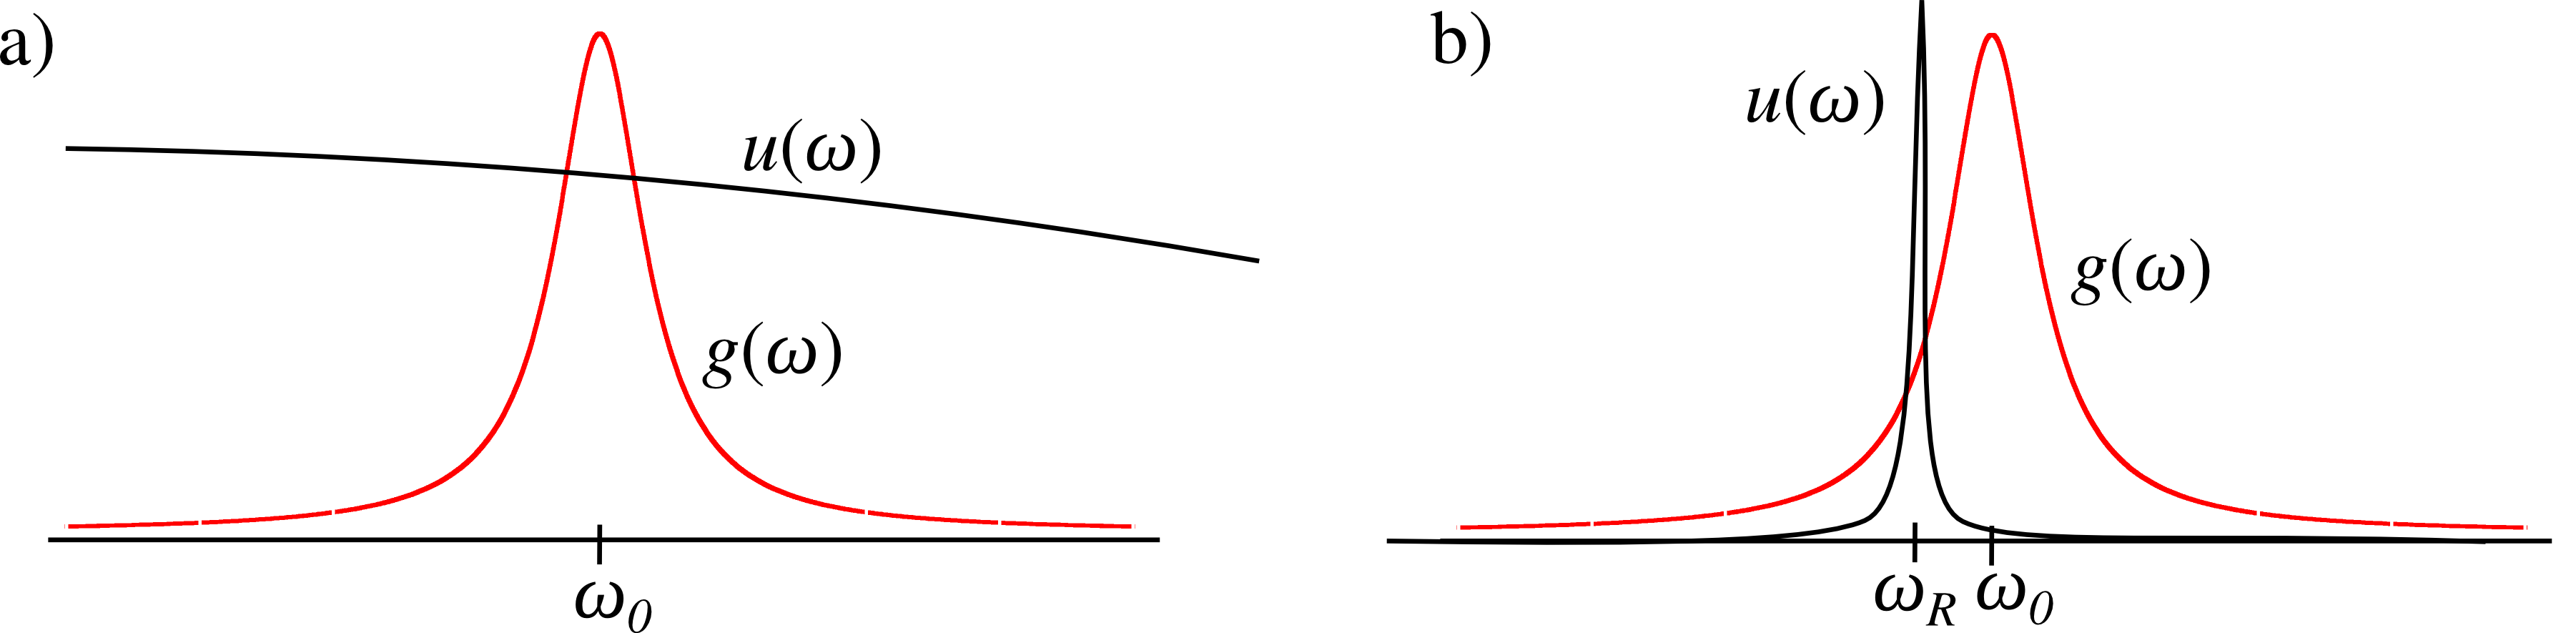
\includegraphics[width=12truecm]{slike/05_Spektri.png}
\caption{Pri izračunu verjetnosti za absorpcijo in stimulirano emisijo je pomembno, ali je 
širina spektralne gostote elektromagnetnega polja bistveno večja (a) ali bistveno manjša (b)
glede na atomsko spektralno črto.}
\label{fig:spektri}
\end{figure}

V splošnem primeru, ko se spekter vpadne svetlobe spreminja v območju 
frekvence prehoda, moramo sešteti prispevke pri posameznih frekvencah (\ref{4.18}) 
po ozkih frekvenčnih intervalih
\begin{equation}
r_{12}=B_{12}\int g(\omega)\, u(\omega)\, d\omega.
\label{4.19}
\end{equation}
Če preverimo gornji zapis na primeru spektra črnega telesa, ki se ne spreminja 
dosti v območju prehoda, lahko $u(\omega)$ postavimo pred integral in po pričakovanju
dobimo znano enačbo~(\ref{4.16}). Iz tega sledi, da mora biti funkcija $g(\omega)$ normirana
\begin{equation}
\int g(\omega)\, d\omega=1.
\label{4.20}
\end{equation}
Zelo pogosto je $g(\omega)$ Lorentzove oblike\index{Spekter!Lorentzov}
\begin{equation}
g(\omega)=\frac{1}{\pi}\frac{\gamma}{(\omega-\omega_{0})^{2}+\gamma^{2}}.
\label{4.21}
\end{equation}
Za grobe ocene lahko funkcijo $g(\omega)$ aproksimiramo tudi s pravokotnikom širine
$\delta\omega\simeq\gamma$ in višine $1/\delta\omega$.

\subsection*{Einsteinovi koeficienti}
\label{AB}
Vrnimo se k fenomenološkim koeficientom $A_{21}$, $B_{21}$ in $B_{12}$, ki jih je 
vpeljal Einstein\footnote{Nemški fizik in nobelovec Albert Einstein, 1879--1955.}. 
S temi koeficienti, pravimo jim tudi Einsteinovi koeficienti\index{Einsteinovi koeficienti}, 
je mogoče uspešno opisati velik del pojavov pri interakciji svetlobe s snovjo.

Vpeljimo pojem zasedenost stanj\index{Zasedenost stanj}, ki pove število 
atomov v določenem stanju. Ker obravnavamo preproste modele atomov z zgolj 
dvema stanjema, zapišemo samo dve zasedenosti. Naj bo $N_1$ zasedenost 
spodnjega stanja, $N_{2}$ zasedenost zgornjega, skupno število atomov pa
$N=N_1+N_2$. V prisotnosti svetlobe 
se bo število atomov v spodnjem in zgornjem stanju v splošnem spreminjalo, skupno 
število pa se bo ohranjalo.

Obravnavajmo termično ravnovesje, ko je spekter svetlobe bistveno širši
od širine atomskega prehoda (slika~\ref{fig:spektri}\,a), tako da lahko
uporabljamo enačbi~(\ref{4.16}) in (\ref{4.17}). Zasedenost zgornjega nivoja
se zmanjšuje zaradi spontanih in stimuliranih prehodov v spodnje
stanje, povečuje pa se zaradi absorpcije s spodnjega stanja. To zapišemo z enačbo
\begin{equation}
\frac{dN_{2}}{dt}=-A_{21}N_2 - r_{21}N_2 + r_{12}N_1 = 
-A_{21}N_{2}-B_{21}u(\omega_{0})N_{2}+B_{12}u(\omega_{0})N_{1}.
\label{4.22}
\end{equation}
Zaradi ohranitve skupnega števila atomov velja 
\beq
\frac{dN_{1}}{dt}=\frac{-dN_{2}}{dt}.
\eeq
V termičnem ravnovesju sta zasedenosti konstantni, tako da lahko zapišemo 
\begin{equation}
\frac{dN_{1}}{dt}=A_{21}N_{2}+B_{21}u(\omega_{0})N_{2}-B_{12}u(\omega_{0})N_{1}=0.
\label{4.23}
\end{equation}
Vemo pa, da mora biti v termičnem ravnovesju spektralna gostota energije sevanja
$u(\omega)$ kar termična Planckova gostota $u_{T}(\omega)$.
Izrazimo najprej spektralno gostoto iz enačbe~(\ref{4.23})
\begin{equation}
u_{T}(\omega_{0})=\frac{A_{21}}{B_{12}\frac{N_{1}}{N_{2}}-B_{21}}.
\label{4.24}
\end{equation}
Vemo tudi, da v termičnem ravnovesju za zasedenosti $N_{1}$ in $N_{2}$ velja
kanonična porazdelitev
\begin{equation}
\frac{N_{2}}{N_{1}}=e^{-\beta(E_{2}-E_{1})} = e^{-\beta \hbar \omega_0},
\label{4.25}
\end{equation}
kjer je $\beta=1/k_BT$. Sledi
\begin{equation}
u_{T}(\omega_{0})=\frac{A_{21}/B_{12}}{e^{\beta\hbar\omega_{0}}-B_{21}/B_{12}}.
\label{4.26}
\end{equation}
Za določitev koeficientov primerjamo gornji izraz s Planckovo formulo za $u_{T}(\omega_{0})$
(enačba~\ref{eq:Planck}). Očitno morata biti koeficienta $B_{21}$ in $B_{12}$ enaka 
(če sta stanji nedegenerirani), med $A_{21}$ in $B_{12}$ pa velja zveza 
\boxeq{4.27}{
A_{21}=\frac{\hbar\omega^{3}}{\pi^{2}c^{3}}\, B_{12} \qquad \mathrm{in} \qquad B_{12}=B_{21}.
}
Koeficient pred $B_{12}$ je ravno enak gostoti stanj elektromagnetnega polja 
$\rho(\omega)$ (enačba~\ref{4.4}), pomnoženi z energijo fotona $\hbar\omega$. 
Videli bomo, da to ni slučajno in da sledi iz verjetnosti za prehod v kvantni 
elektrodinamiki (poglavje~\ref{chap:verjetnost}).
Pozoren bralec je lahko tudi opazil, da je z enačbo~(\ref{4.26}),
ki smo jo dobili le z uporabo kanonične porazdelitve za atome, že
določena oblika Planckove formule, ne da bi karkoli rekli o fotonih.

\section{Absorpcijski koeficient}

V prejšnjem razdelku smo napovedali, da lahko velik del pojavov pri interakciji 
svetlobe s snovjo opišemo z Einsteinovimi koeficienti. Poskusimo zdaj 
koeficienta $A_{21}$ in $B_{21}$ povezati z makroskopskim absorpcijskim
koeficientom plina atomov. 

Naj na izbran volumen plina vpada snop svetlobe s frekvenco
$\omega$, ki je blizu frekvence atomskega prehoda $\omega_{0}$. Gostota
vpadnega energijskega toka je $j_{\omega}=w_{\omega}c$ (enačba~\ref{eq:jcw}), 
pri čemer je $w_{\omega}$ gostota energije. Obravnavajmo primer, ko je 
spekter vpadnega snopa ozek v primerjavi s širino atomskega prehoda
(slika~\ref{fig:spektri}\,b). V tej obliki zapisane enačbe bodo bolj 
priročne pozneje pri obravnavi laserja. Privzemimo še, da
je stanje stacionarno. 
\begin{figure}[h]
\centering
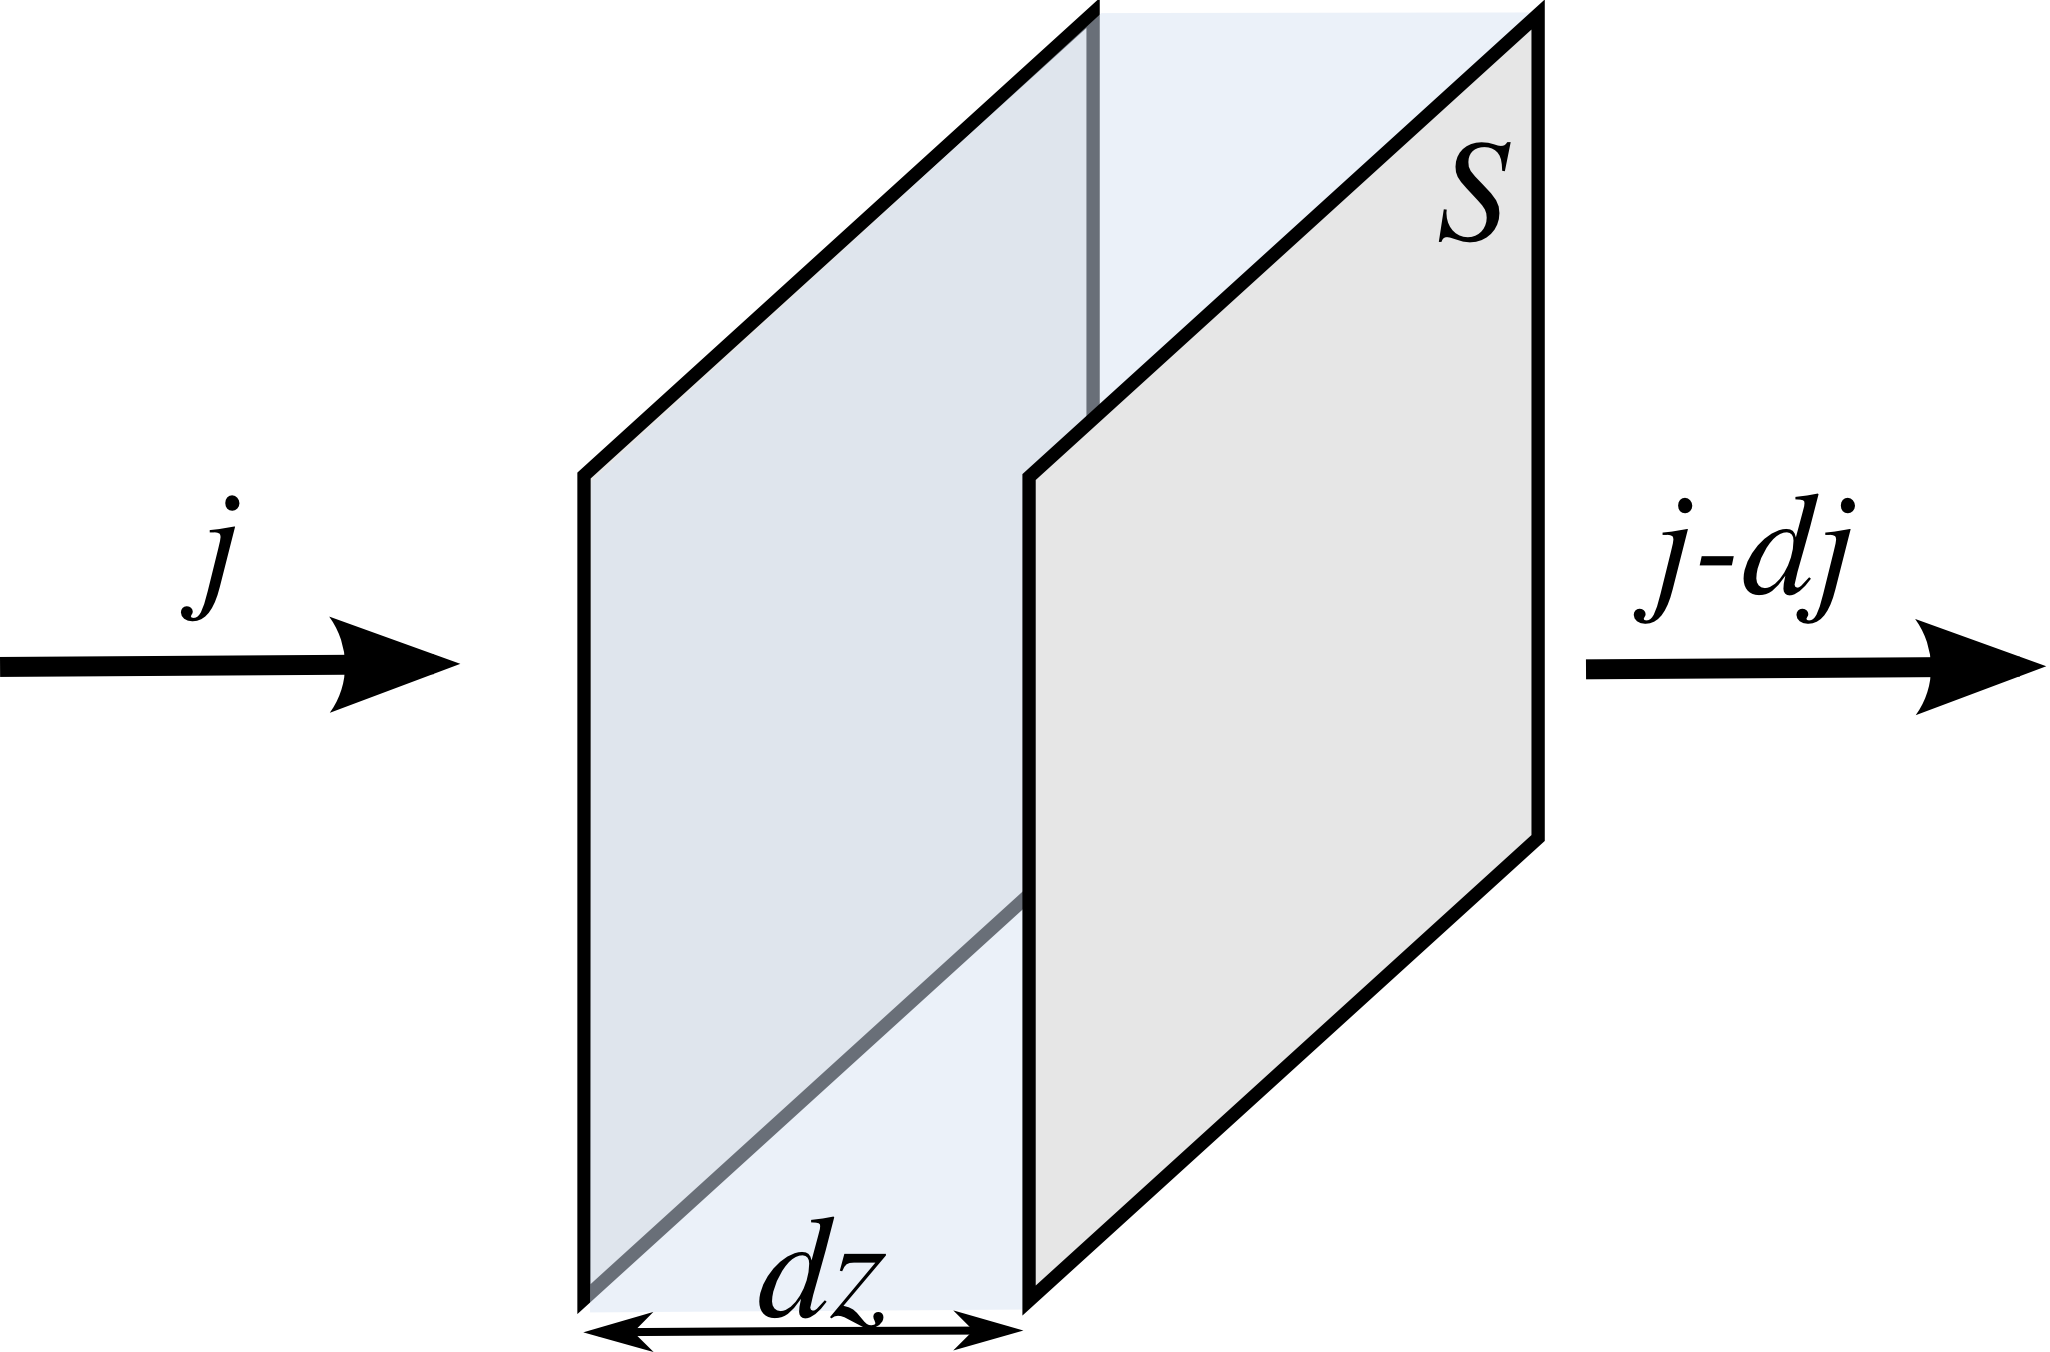
\includegraphics[width=6truecm]{slike/05_Absorpcija.png}
\caption{K absorpciji snopa svetlobe v plasti atomov}
\label{fig:abs}
\end{figure}
 
Ko svetloba vpade na plast plina debeline $dz$, se gostota
energijskega toka zmanjša zaradi absorpcije in hkrati poveča zaradi 
stimulirane emisije (slika~\ref{fig:abs}). 
Spontano sevanje, ki je seveda tudi prisotno, lahko zanemarimo, saj
bo izsevano na vse strani enakomerno in ga bo le zelo majhen del v smeri snopa.
Sprememba energije snopa na enoto časa je enaka razliki med 
številom absorpcij in stimuliranih prehodov na enoto časa, pomnoženih z 
energijo fotona. To popišemo z enačbo 
\begin{equation}
dP=S\, dj=(N_{2}-N_{1}) \, \frac{S dz}{V} \, \hbar\omega \,r_{12} = 
(N_{2}-N_{1})\, \frac{S dz}{V}\, \hbar\omega \, B_{21}g(\omega) w_{\omega},
\label{4.28}
\end{equation}
pri čemer smo verjetnost z prehod izrazili iz enačbe~(\ref{4.18}).
S $S$ smo označili presek snopa, z $V$ pa volumen plina. Tako dobimo 
enačbo za spreminjanje gostote toka 
\begin{equation}
dj=\frac{1}{V}(N_{2}-N_{1})\, B_{21}g(\omega)\, \frac{\hbar\omega}{c}j_{\omega}\, dz
\label{4.29}
\end{equation}
Priročno je vpeljati še presek za absorpcijo\index{Presek za absorpcijo} ali
stimulirano sevanje\index{Presek za stimulirano sevanje} 
\beq
\sigma(\omega)=\frac{B_{21}\, g(\omega)\, \hbar\omega}{c}.
\label{sigma}
\eeq
Z njim se izraz (\ref{4.29}) poenostavi v 
\boxeq{4.30}{
\frac{dj}{dz}=\frac{N_{2}-N_{1}}{V}\sigma(\omega)j.
}
Navadno imamo opravka s plinom, ki je blizu termičnega ravnovesja,
zato je $N_{2}<N_{1}$ in je $dj$ negativen. V tem primeru pride do
absorpcije\index{Absorpcija} z absorpcijskim koeficientom\index{Absorpcijski koeficient}
\begin{equation}
\mu(\omega)=\frac{N_{1}-N_{2}}{V}\, B_{21}\, g(\omega)\frac{\hbar\omega}{c}=
\frac{N_{1}-N_{2}}{V}\sigma(\omega),
\label{4.31}
\end{equation}
za gostoto energijskega toka pa velja enačba
\beq
\frac{dj}{j} = -\mu dz.
\label{eq:jabs}
\eeq
Energija se pri absorpciji na našem plinu dvonivojskih atomov seveda
ne izgublja, temveč le siplje. Atom, ki je prešel v vzbujeno stanje,
se s spontano emisijo vrne nazaj v osnovno, svetloba pa se izseva
na vse strani -- se siplje.

\section{Nasičenje absorpcije}
\label{chap:NasAbs}

Čeprav je na prvi pogled enačba~(\ref{eq:jabs}) za zmanjševanje 
gostote svetlobnega toka pri prehodu skozi absorbirajoči plin preprosta,
je ni mogoče enostavno integrirati, saj je $\mu$ odvisen od 
gostote energijskega toka. Pri dovolj veliki gostoti
svetlobnega toka namreč z absorpcijo znaten delež
atomov preide v višje stanje, zaradi česar se zmanjša razlika $N_{1}-N_{2}$,
posledično se pa zmanjša tudi absorpcijski koeficient -- absorpcija
se nasiti. Zato temu pojavu pravimo nasičenje absorpcije\index{Nasičena absorpcija}.
Obravnavajmo ga še matematično.

Obravnavajmo snop monokromatske svetlobe, ki vpada na plin. 
Atomi v plinu prehajajo med nivoji zaradi absorpcije, spontane in stimulirane emisije. 
Podobno kot smo zapisali enačbo~(\ref{4.23}) za termično ravnovesje v primeru
širokega spektra, zapišemo stacionarno enačbo za naš primer kot
\begin{equation}
A_{21}N_{2}+B_{21}\,g(\omega)\,(N_{2}-N_{1})\frac{j}{c}=0,
\label{4.32}
\end{equation}
pri čemer smo za verjetnost za prehod namesto enačbe~(\ref{4.17}) vzeli
enačbo~(\ref{4.18}). Zasedenost višjega stanja $N_{2}$ lahko izrazimo s 
celotnim številom atomov $N$ in razliko zasedenosti 
\beq
N_{2}=\frac{1}{2}N+\frac{1}{2}(N_{2}-N_{1}).
\label{4.321}
\eeq
S tem lahko izračunamo razliko zasedenosti 
\begin{equation}
N_{2}-N_{1}=-\frac{N}{1+2\frac{Bg(\omega)}{cA}j}.
\label{4.33}
\end{equation}
Pri majhni gostoti toka $j$ so praktično vsi atomi v osnovnem stanju in prispevajo
k absorpciji. Pri velikih gostotah toka pa imenovalec gornjega
izraza močno naraste, razlika zasedenosti gre proti nič in absorpcija se zmanjšuje.
Ko drugi člen v imenovalcu enačbe~(\ref{4.33}) doseže vrednost 1, pravimo, da
gostota energijskega toka doseže vrednost saturacijske gostote\index{Saturacijska gostota toka}.
Zapišemo jo kot 
\begin{equation}
j_{s}(\omega)=\frac{cA_{21}}{2B_{21}g(\omega)}=
\frac{\hbar\omega^{3}}{2\pi^{2}c^{2}g(\omega)},
\label{4.34}
\end{equation}
pri čemer smo upoštevali zvezo~(\ref{4.27}) med koeficientoma $A_{21}$ in $B_{21}$.
Kot vidimo, je saturacijska gostota odvisna le od frekvence vpadnega valovanja 
in širine atomskega prehoda. Za črto z valovno dolžino okoli 600~nm in širino črte
$10^{8}~\mathrm{s}^{-1}$ znaša saturacijska gostota svetlobnega toka okoli 
$20~\mathrm{mW/cm}^{2}$. Tako gostoto toka v ozek frekvenčni interval
je z običajnimi svetili, na primer plinsko razelektritveno cevjo,
praktično nemogoče doseči, medtem ko jo iz laserjev dobimo z lahkoto.
Izraz za razliko zasedenosti stanj lahko zdaj zapišemo v pregledni obliki
\begin{equation}
N_{2}-N_{1}=-\frac{N}{1+\frac{j}{j_{s}(\omega)}}.
\label{4.35}
\end{equation}
Vstavimo gornji izraz v enačbo za zmanjševanje gostote toka (enačba~\ref{4.30}) in 
dobimo 
\boxeq{4.36}{
dj=-\frac{\mu_{0}}{1+\frac{j}{j_{s}}}\, j\, dz,
}
kjer smo z $\mu_{0}=N\,B_{21}\,g(\omega)\,\hbar\omega/Vc$ označili
absorpcijski koeficient pri majhnih gostotah vpadnega toka.
Enačbo brez težav integriramo in dobimo 
\begin{equation}
\ln\frac{j}{j_{0}}+\frac{1}{j_{s}}(j-j_{0})=-\mu_{0}\, z,\label{4.37}
\end{equation}
kjer smo z $j_{0}$ označili začetno gostoto toka. 
\begin{figure}[h]
\centering
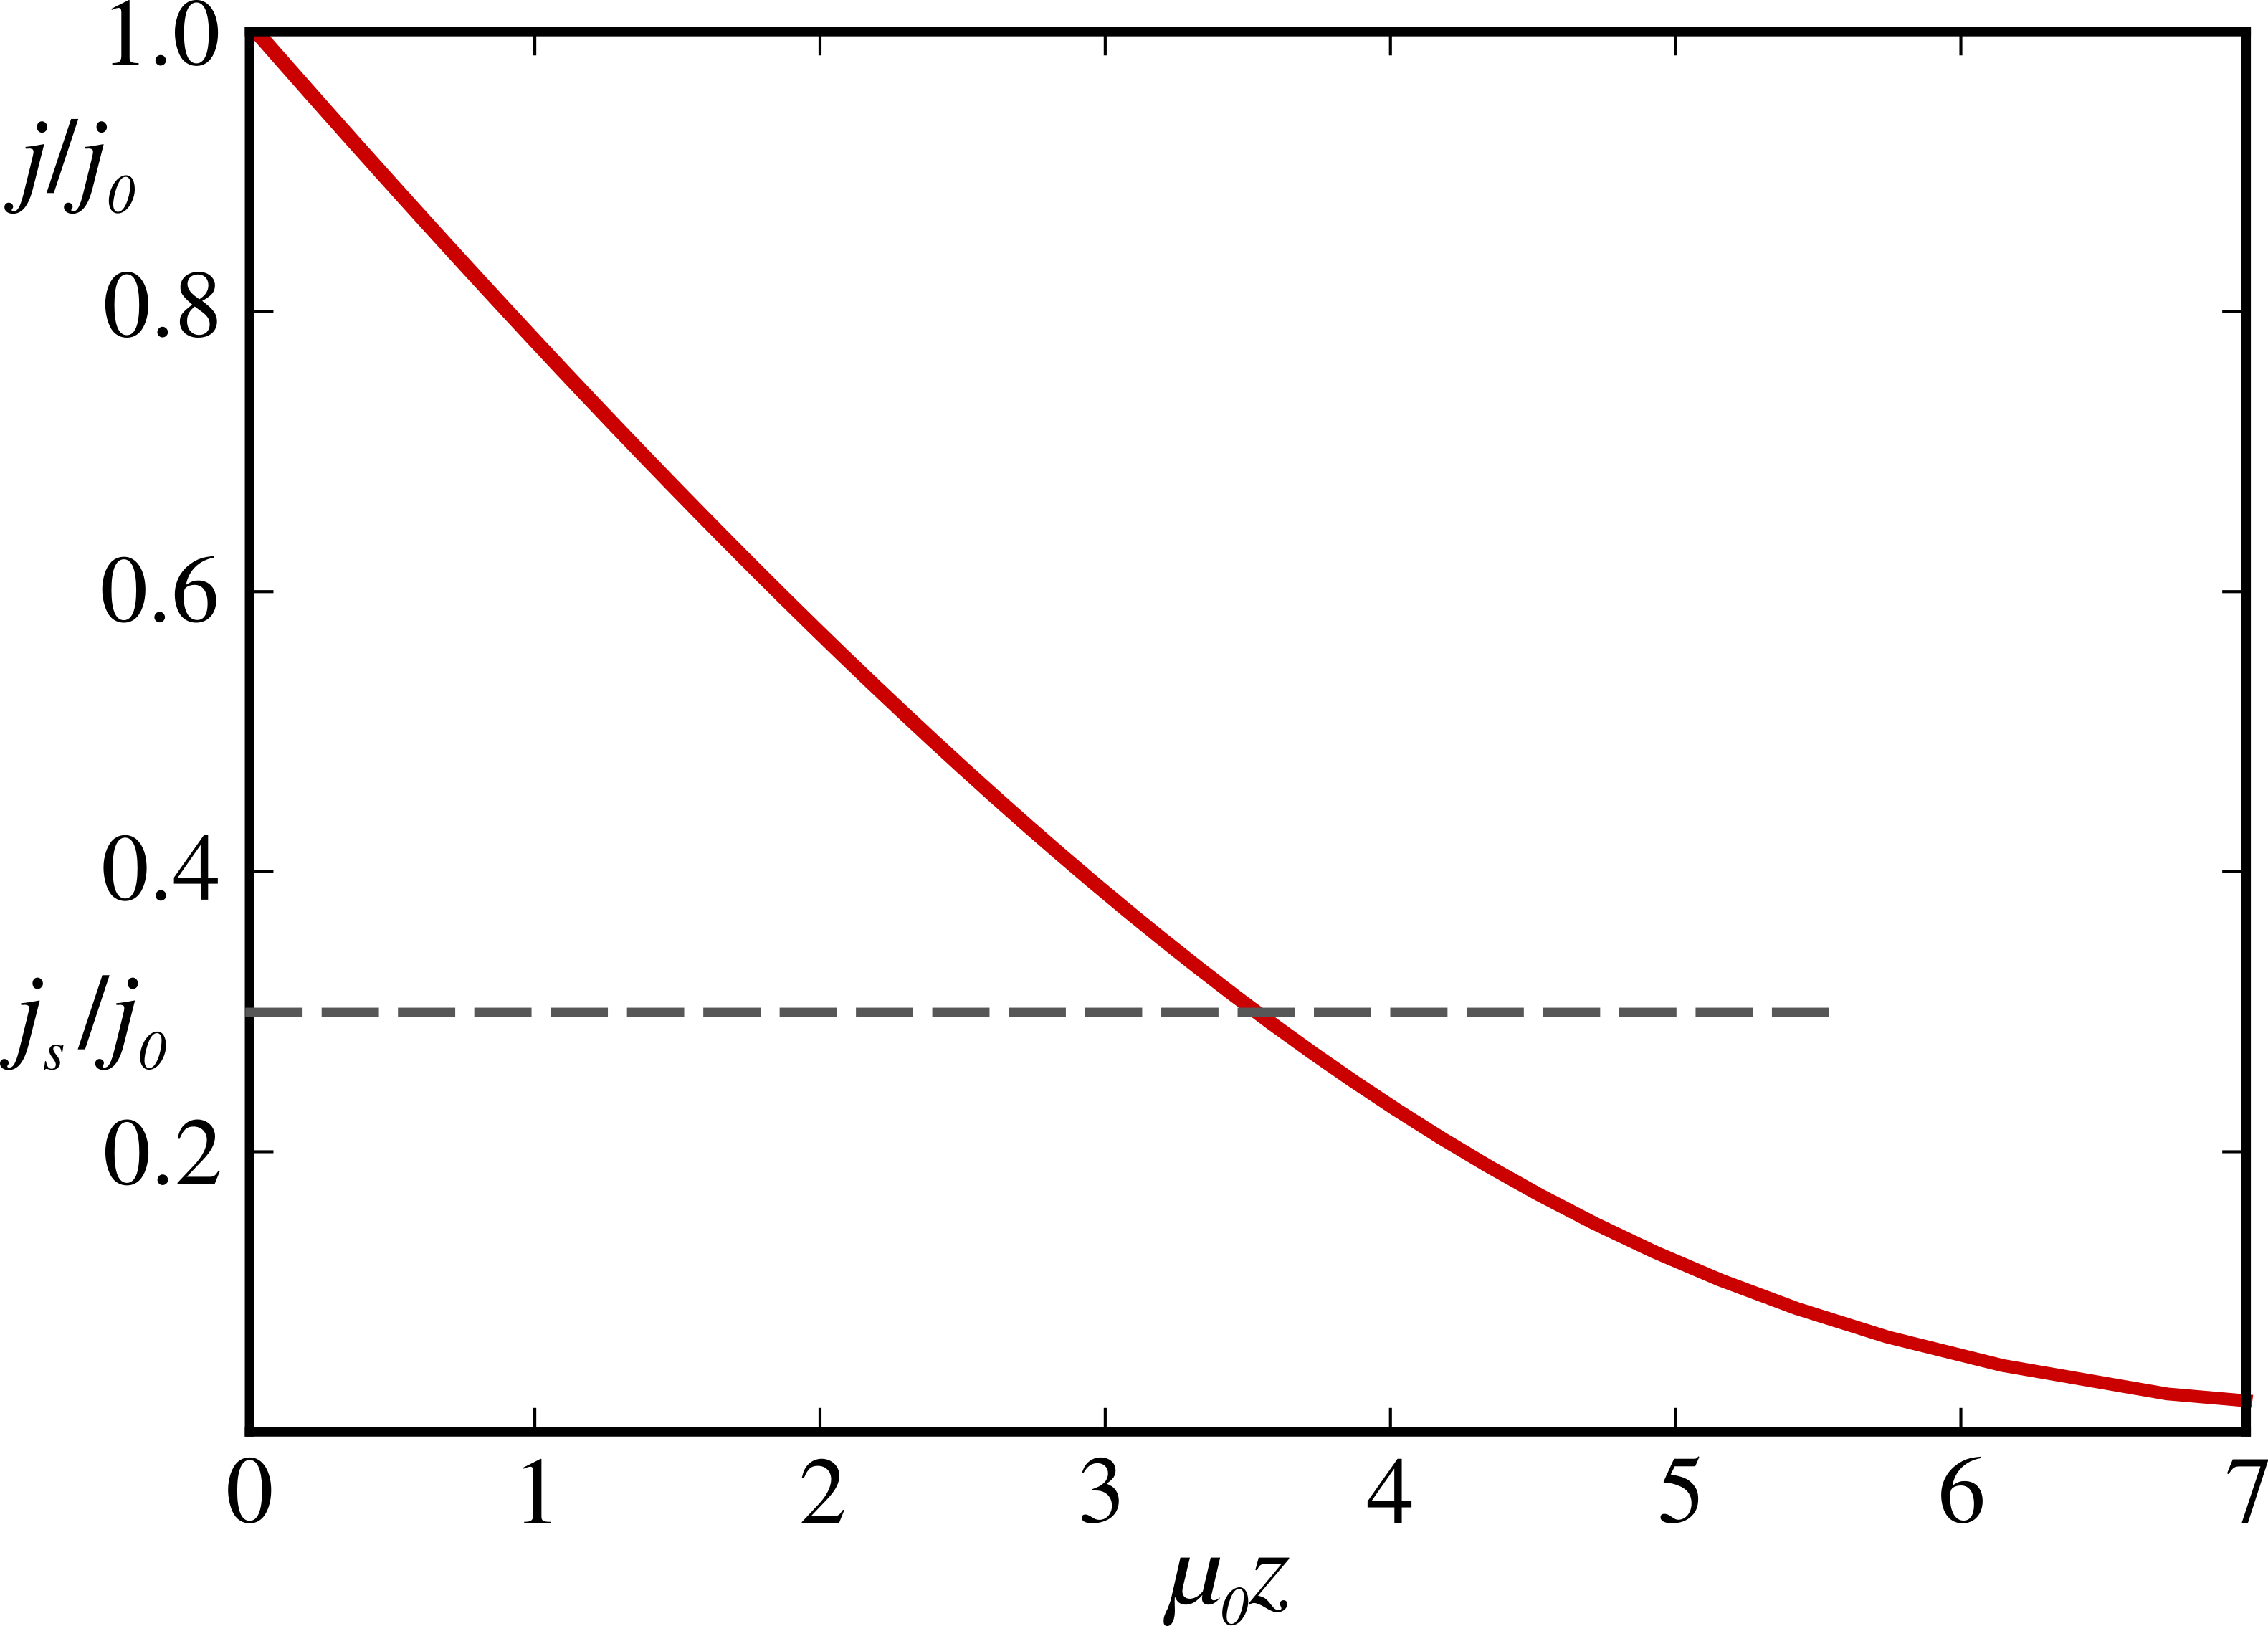
\includegraphics[width=8truecm]{slike/05_jabs.png}
\caption{Pojemanje gostote svetlobnega toka v absorbirajočem plinu}
\label{fig:abs2}
\end{figure}
Kadar je ta dosti
manjša od $j_{s}$, lahko drugi člen v gornji enačbi zanemarimo in dobimo 
navadno eksponentno pojemanje
\beq
j = j_0 e^{-\mu_0 z}.
\eeq
Pri zelo velikih vpadnih gostotah pa lahko zanemarimo prvi člen in dobimo, 
da je pojemanje zgolj linearno
\begin{equation}
j=j_{0}-\mu_{0}j_{s}z=j_{0}-\frac{N}{2V}A\hbar\omega\, z.
\label{4.38}
\end{equation}
V primeru močnega vpadnega toka je zasedenost spodnjega in zgornjega nivoja skoraj
enaka in je absorpcija omejena s tem, kako hitro se atomi vračajo
v osnovno stanje preko spontanega sevanja, kar je razvidno tudi iz
zadnje oblike izraza~(\ref{4.38}).

\section{Optično ojačevanje}
V prejšnjih razdelkih smo obravnavali prehod svetlobe skozi dvonivojski plin. V primeru
termičnega ravnovesja je zgornji nivo manj zaseden od spodnjega in v plinu pride
do absorpcije svetlobe. Če pa nekako dosežemo primer, da je $N_{2}>N_{1}$, 
se bo snop svetlobe pri prehodu skozi tako pripravljen plin ojačeval. 
Takemu primeru pravimo stanje obrnjene zasedenosti\index{Obrnjena zasedenost}. 
Tako stanje seveda ni v termičnem ravnovesju in ga je treba vzdrževati z dovajanjem 
energije plinu. Dovajanju energije pravimo tudi črpanje\index{Optično črpanje}. 
Načinov, kako dosežemo obrnjeno zasedenost s črpanjem je veliko. Oglejmo 
si nekaj primerov. 

V plinih je najpogostejši način vzbujanja z električnim tokom. Elektroni,
ki so glavni nosilci toka, se zaletavajo v atome ali ione in jih vzbujajo
na višje nivoje, pri čemer lahko pride do obrnjene zasedenosti med
nekim parom nivojev. Pogost proces v plinih je tudi prenos energije
med atomi s trki. Vzemimo mešanico dveh plinov, pri katerih se nek
nivo enih atomov ujema po energiji s stanjem drugih atomov. Vzbujen
atom prve vrste lahko pri trku preda energijo brez sevanja atomu druge
vrste, ki iz osnovnega stanja preide v ustrezen višji nivo. Če je
pod tem nivojem še drugo vzbujeno stanje, bomo med njima dobili obrnjeno
zasedenost, kadar je življenjski čas gornjega nivoja daljši od spodnjega.

V trdnih neprevodnih kristalih sta v optičnem področju absorpcija
in sevanje pri določeni valovni dolžini navadno posledica primesi.
Obrnjeno zasedenost para nivojev primesi največkrat dobimo tako, da
kristal obsevamo s svetlobo s frekvenco, ki ustreza prehodu na nek
nivo nad izbranim parom. Tak način optičnega črpanja deluje tudi v
organskih barvilih.

V polprevodnikih dosežemo obrnjeno zasedenost med prevodnim in valenčnim
pasom z vbrizgavanjem elektronov in vrzeli v območje p-n spoja z električnim
tokom v prevodni smeri. Možen mehanizem vzbujanja so tudi kemične
reakcije. Po reakciji lahko produkti ostanejo v vzbujenem stanju
in lahko dobimo obrnjeno zasedenost med paroma stanj.

Nekoliko bolj podrobno si bomo nekaj teh mehanizmov ogledali v nadaljevanju
na konkretnih laserjih. Zaenkrat si kot primer oglejmo le model optičnega
črpanja plina atomov s tremi stanji.

\section{Optično črpanje trinivojskega sistema}

Naj imajo atomi poleg osnovnega stanja z energijo $E_0$, označimo ga $|0\rangle$,
še dve vzbujeni stanji z energijo $E_1$ (stanje $|1\rangle$) in energijo $E_2>E_1$
(stanje $|2\rangle$). Na plin svetimo s svetlobo, ki
vzbuja atome iz stanja $|0\rangle$ v stanje $|2\rangle$, pri čemer
je lahko spektralna gostota $u_{p}$ črpalne svetlobe široka. Poleg
tega naj se po plinu širi še monokromatska svetloba s frekvenco $\omega$
blizu frekvence prehoda $\omega_{0}$ med stanjema $|1\rangle$ in
$|2\rangle$ in z gostoto energije $w$. Ugotoviti želimo, pri kakšnih
pogojih lahko dosežemo obrnjeno zasedenost med stanjema $|1\rangle$ in $|2\rangle$
in s tem ojačevanje svetlobe okoli frekvence $\omega_{0}$.
\begin{figure}[h]
\centering
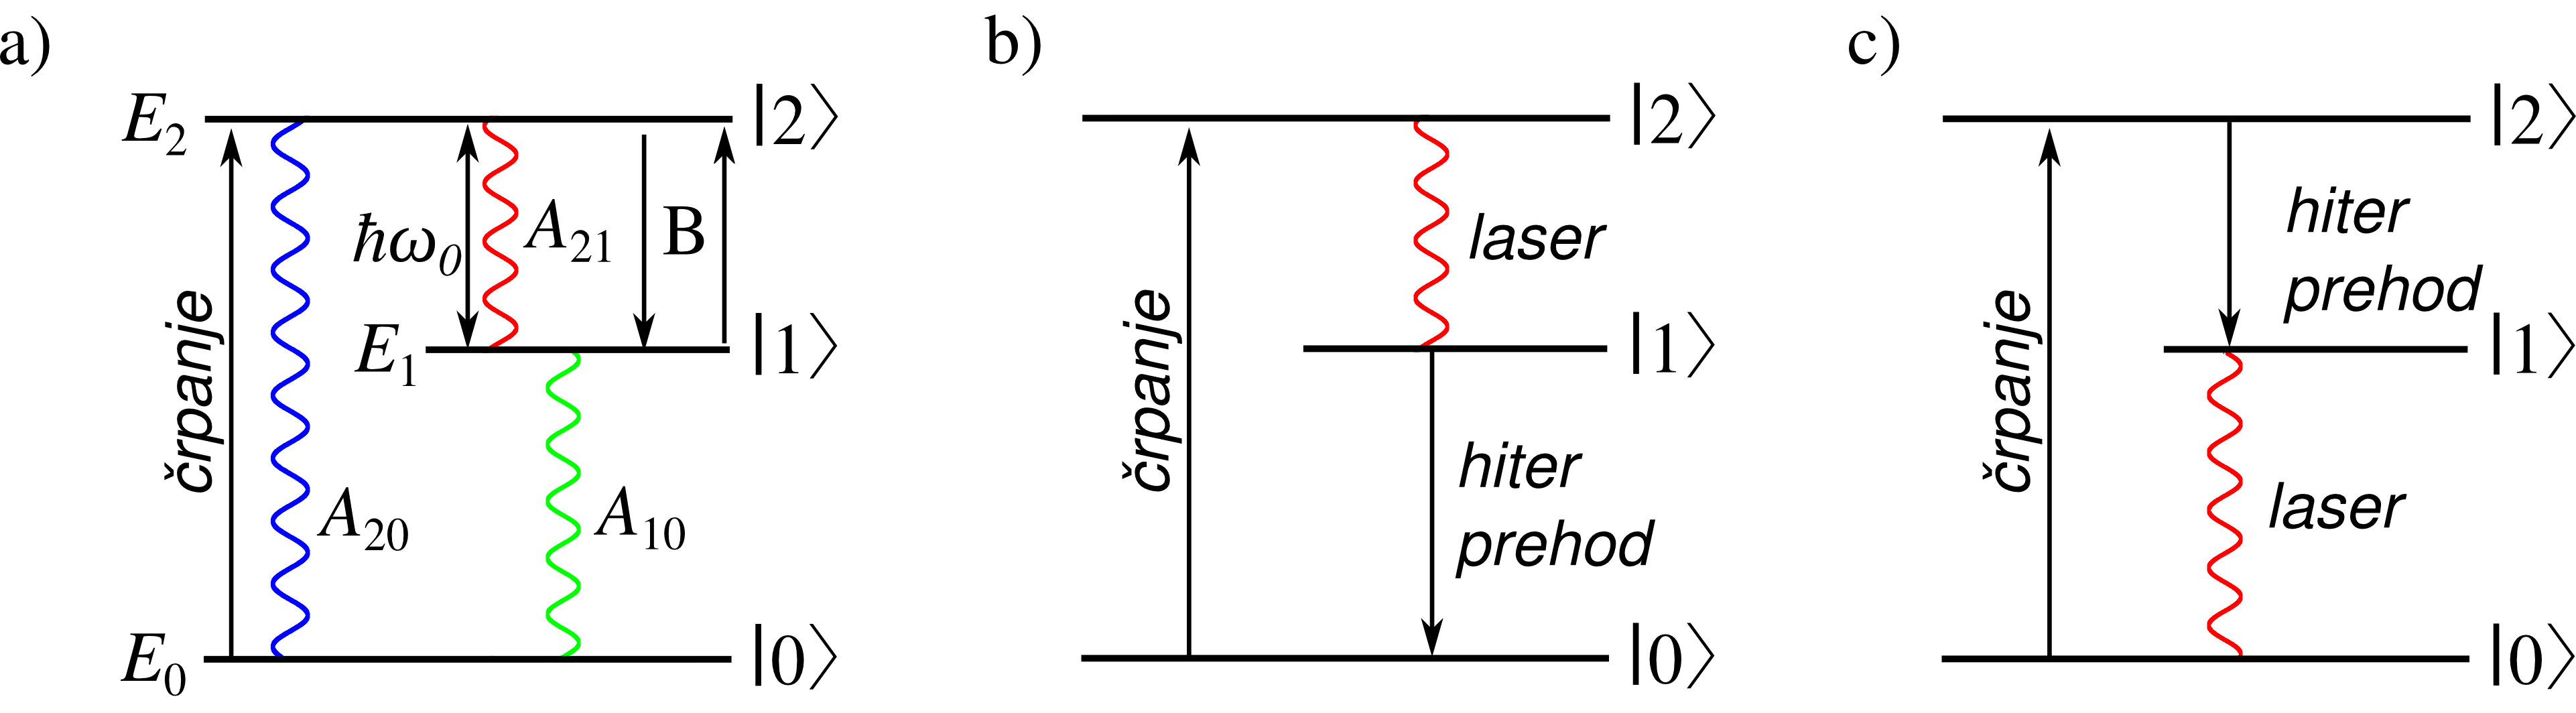
\includegraphics[width=14truecm]{slike/05_Trinivojski.png}
\caption{Shema energijskih nivojev trinivojskega sistema in prehodov med njimi (a).
V plinskih laserjih imamo navadno stanje obrnjene zasedenosti med drugim in prvim
vzbujenim stanjem (b), v navadnih trdninskih laserjih (npr. rubinskem) pa med 
prvim vzbujenim in osnovnim stanjem (c).}
\label{fig:3nivojski}
\end{figure}

Zapišimo enačbe za spreminjanje zasedenosti posameznih stanj. Osnovno stanje
se prazni zaradi absorpcije črpalne svetlobe in polni zaradi
spontanih prehodov iz stanj $|1\rangle$ in $|2\rangle$, stimulirane
prehode iz stanja $|2\rangle$ pa bomo zanemarili. Zasedenost stanja $|2\rangle$ se
povečuje zaradi absorpcije s spodnjih nivojev in zmanjšuje
zaradi spontanega in stimuliranega sevanja. Srednje stanje se polni
s stimuliranimi in spontanimi prehodi iz stanja $|2\rangle$ in prazni
zaradi absorpcije v $|2\rangle$ in spontanih prehodov v $|0\rangle$.
Pri tem velja, da je vsota vseh treh zasedenosti enaka številu vseh atomov: $N_{0}+N_{1}+N_{2}=N$. 
Zasedbene enačbe so torej 
\begin{eqnarray}
\frac{dN_{0}}{dt} & = & -rN+A_{20}N_{2}+A_{10}N_{1} \label{4.39.1}\\
\frac{dN_{1}}{dt} & = & -A_{10}N_{1}+B_{21}\,g(\omega)\,w\, (N_{2}-N_{1})+A_{21}N_{2} \label{4.39.2}\\
\frac{dN_{2}}{dt} & = & rN_0-A_{20}N_{2}-A_{21}N_{2}+B_{21}\,g(\omega)\,w\, (N_1-N_2),
\label{4.39}
\end{eqnarray}
pri čemer predpostavili, da je $N_0 \approx N \gg N_1, N_2$ in zato lahko črpanje $B_{20}\, 
u_{p} (N_0-N_2)$, ki je praktično konstantno, zapisali s koeficientom $r$. Mehanizem črpanja 
smo tako skrili v $r$ in prav nič ni pomembno, na kakšen način poteka. 

Zanima nas stacionarno stanje, ko so vsi trije časovni odvodi enaki nič. 
Brez škode lahko tudi zanemarimo spontano sevanje iz stanja
$|2\rangle$ v osnovno stanje. Tako iz druge enačbe sistema~(\ref{4.39.2}) 
dobimo
\begin{eqnarray}
B_{21}\,g(\omega\,)w\, N_{2}+A_{21}N_{2} = B_{21}\,g(\omega\,)w\, N_{1} + A_{10}N_{1} 
\end{eqnarray}
in
\begin{eqnarray}
N_2 = \frac{B_{21}\,g(\omega\,)w + A_{10}}{B_{21}\,g(\omega\,)w+A_{21}}N_1.  
\end{eqnarray}
Ob upoštevanju zveze, ki jo dobimo iz prve enačbe sistema~(\ref{4.39.1})
\beq
N_1= \frac{rN}{A_{10}}, 
\eeq
zapišemo razliko zasedenosti kot 
\begin{equation}
N_{2}-N_{1}=\left(\frac{N_2}{N_1}-1\right)N_1=\frac{A_{10}-A_{21}}{A_{21}+
B_{21}g(\omega)w} \,\frac{rN}{A_{10}}.
\label{4.42}
\end{equation}
Iz gornje enačbe sledi, da dobimo obrnjeno zasedenost, če je $A_{10}>A_{21}$, torej kadar je
razpadni čas stanja $|1\rangle$ krajši kot razpadni čas stanja $|2\rangle$.
Tak rezultat smo seveda lahko pričakovali.

V praktični primerih navadno velja $A_{10}\gg A_{21}$. Ob upoštevanju zveze $j=wc$ povežemo
razliko zasedenosti z gostoto vpadnega svetlobnega toka
\beq
N_{2}-N_{1}=\frac{rN}{A_{21}} \, \frac{1}{1+\frac{B_{21}g(\omega)j}{c A_{21}}} = 
\frac{rN}{A_{21}} \, \frac{1}{1+j/j_s}.
\label{eq:3n_N}
\eeq
Konstante $c A_{21}/B_{21}g(\omega)$ smo pospravili v $j_s$, ki ga bomo imenovali 
saturacijska gostota svetlobnega toka\index{Saturacijska gostota toka}. Vidimo, da je dobljen
izraz zelo podoben saturacijski gostoti za dvonivojski sistem (enačba~\ref{4.34}), razlika je le
v faktorju 2. Do te razlike pride zaradi različnega števila stanj in pogoj $N_{1}+N_{2}=N$
ne velja več. 

\begin{definition}
 Pokaži, da je saturacijska gostota toka $j_2$ odvisna le od frekvence valovanja in širine 
 atomske črte $\delta \omega$. 
\end{definition}

Poglejmo zdaj, kaj se ob vpadu na plast trinivojskega plina zgodi s svetlobo s frekvenco $\omega$ in 
gostoto svetlobnega toka $j=wc$. Račun je zelo podoben računu pri absorpciji (enačba~\ref{4.29}). Zapišemo
spremembo gostote toka na debelini $dz$ 
\begin{equation}
dj=\frac{1}{V}(N_{2}-N_{1})\, B_{21}g(\omega)\, \frac{\hbar\omega}{c}j\, dz,
\label{eq:dj}
\end{equation}
pri čemer gostota toka $j = wc$ nastopa tudi v izrazu za razliko zasedenosti (enačba~\ref{eq:3n_N}). 
Če to upoštevamo, dobimo diferencialno enačbo za gostoto toka
\begin{equation}
\frac{1}{j}\left(1+\frac{j}{j_{s}}\right)\, dj=G\, dz
\label{4.43}
\end{equation}
oziroma
\boxeq{eq:djG}{
dj=\frac{G}{1+\frac{j}{j_{s}}}\, j\, dz,
}
ki je spet zelo podobna enačbi za absorpcijo (enačba~\ref{4.36}).
Z $G$ smo označili t.i. koeficient ojačenja pri majhnih vpadnih gostotah
toka. Podan je z 
\begin{equation}
G=\frac{rNB_{21}\hbar\omega g(\omega)}{VcA_{21}}.\label{4.44}
\end{equation}
Rešitev diferencialne enačbe je prikazana na sliki~(\ref{fig:ojacanje}). 
\begin{figure}[h]
\centering
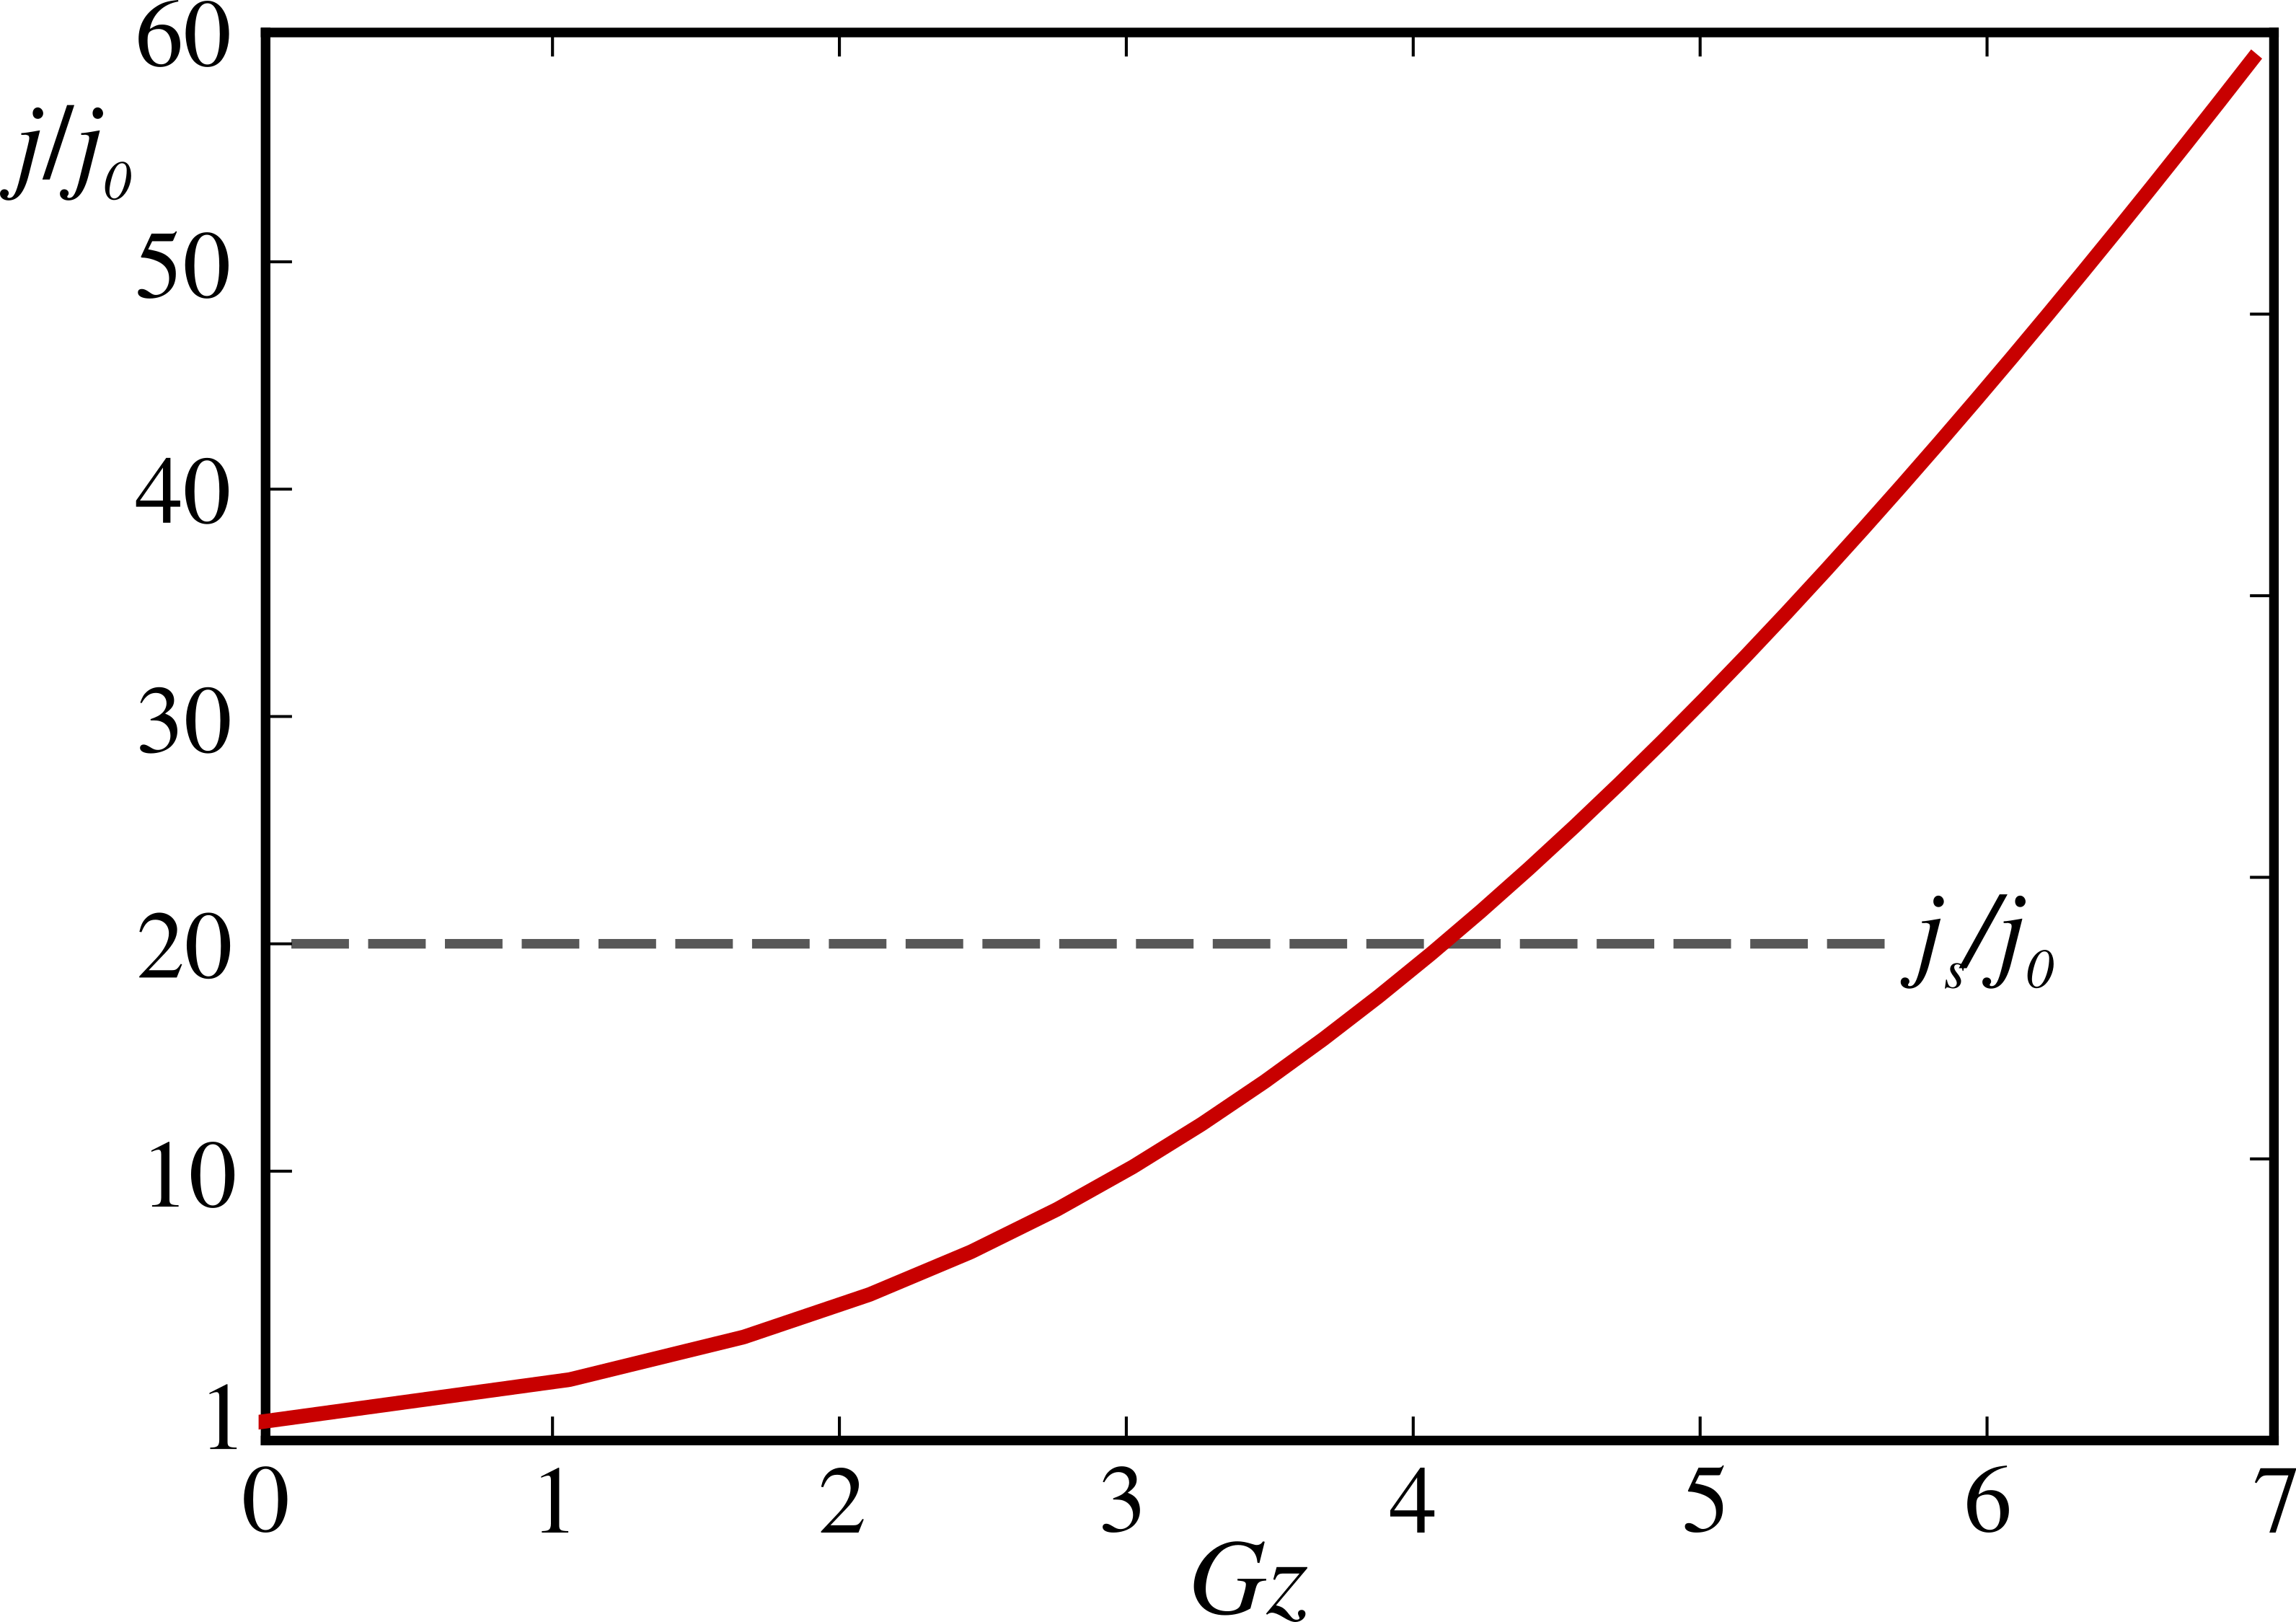
\includegraphics[width=8truecm]{slike/05_joja.png}
\caption{Naraščanje gostote svetlobnega toka pri optičnem ojačanju}
\label{fig:ojacanje}
\end{figure}

Obnašanje gostote svetlobnega toka ima, tako kot pri absorpciji, dva režima. 
Pri majhnih gostotah toka $j\ll j_{s}$ je naraščanje eksponentno 
\begin{equation}
j(z)=j_{0}e^{Gz}.
\label{4.45}
\end{equation}
Pri velikih gostotah toka pride do nasičenja in gostota svetlobnega
toka se ojačuje linearno z razdaljo
\begin{equation}
j(z)=\tilde{j_{0}}+j_{s}Gz=\tilde{j_{0}}+\frac{rN}{V}\hbar \omega z.
\label{4.46}
\end{equation}
 V tem primeru je gostota toka dovolj velika, da vsi atomi, ki jih
s črpanjem spravimo v najvišje stanje, preidejo v stanje $|1\rangle$
s stimuliranim sevanjem. Pri konstantnem črpanju je tedaj 
linearno naraščanje gostote toka razumljivo. 

\section{Homogena in nehomogena razširitev spektralne črte}
\label{Razsiritev}
Doslej smo predpostavili, da svetijo vsi atomi obravnavane snovi
pri isti frekvenci $\omega_{0}$ in z isto spektralno širino, ki smo
jo popisali s funkcijo $g(\omega)$, z vrhom pri $\omega_0$. Če to drži, 
pravimo, da je razširitev spektralne črte homogena\index{Spektralna črta!homogena razširitev}. 
Primera homogene razširitve sta naravna širina in razširitev zaradi trkov med atomi. 
Funkcija $g(\omega)$ je v tem primeru Lorentzove oblike
\beq
g(\omega)=\frac{1}{\pi}\frac{\gamma}{(\omega-\omega_{0})^{2}+\gamma^{2}}
\eeq
s širino črte $\gamma$. 

% %izračunaj širino zaradi trkov v HeNE laserju. Tlak p, molska masa M, 
% collision time tc sqrt(2/3 MkT)/8 pi pa^2.
% pri 0.5 atm, tc 0.5 mus, delta ni 0.64 MHz << 5 10^14 hz. 
% Primerjaj z naravno širino, = kako sešteješ.
% 
% Nehomogena razširitev - Gauss, impurities v steklu, local elektctic field, 
% Stark shift, NdGlass, 5.4 THz, 
% 
% Doppler / Gauss.HenE 1.7 GHz
% 
% Seštevanje razširitev s konvolucijo int g*(x) g(omega - omega 0-x) dx
% voigt funkcija
% če dva homogena, delta je vsota delta.
% če dva nehomogena delata je sqrt delta^2

Spektralna črta je lahko razširjena tudi zato, ker vsi atomi ne svetijo
pri povsem enaki frekvenci. Tedaj govorimo o nehomogeni 
razširitvi\index{Spektralna črta!nehomogena razširitev}.
Najpomembnejši primer nehomogene razširitve je Dopplerjeva 
\index{Dopplerjeva razširitev} razširitev v plinu. 
Atomi plina vedno sevajo pri praktično isti frekvenci, vendar jih zaradi gibanja
opazovalec v mirujočem (laboratorijskem) sistemu v skladu z Dopplerjevim pojavom 
zazna pri različnih frekvencah. Tako so frekvence $\omega$ posameznih atomov 
odvisne od hitrosti $v$ atoma glede na smer opazovanja. Zapišemo jih kot  
\begin{equation}
\omega=\omega_{0}-\frac{v}{c}\omega_{0}=\omega_{0}-k_{0}v.
\label{4.81}
\end{equation}
Označimo z ${\cal N}(v)$ porazdelitev gostote atomov po hitrostih
v smeri opazovanja. V termičnem ravnovesju je ${\cal N}(v)$ Maxwellova
porazdelitev
\begin{equation}
{\cal N}(v)=\frac{N}{V}\left(\frac{m}{2\pi k_{B}T}\right)^{1/2}e^{-\frac{mv^{2}}{2k_{B}T}}.
\label{4.82}
\end{equation}
 Porazdelitev atomov po frekvencah dobimo tako, da hitrost izrazimo
iz enačbe~(\ref{4.81}), pri čemer dobljeno funkcijo $g_{D}(\omega)$
normiramo tako. Dobimo
\begin{equation}
g_{D}(\omega)=\frac{c}{\omega_{0}}\left(\frac{m}{2\pi 
k_{B}T}\right)^{1/2}e^{-\frac{mc^{2}}{2k_{B}T}\frac{(\omega-\omega_{0})^{2}}{\omega_{0}}}.
\label{4.821}
\end{equation}
Dopplerjeva razširitev v plinu je torej Gaussove oblike. Njena širina pri polovični 
višini\footnote{To širino imenujemo FWHM -- \it{Full width at half maximum}.} je
\begin{equation}
\Delta\omega_{D}=2 \sqrt{\frac{2k_{B}T \ln 2}{mc^{2}}}\omega_{0}.
\label{4.83}
\end{equation}
\begin{definition}
Izpelji obliko nehomogeno razširjene črte za Dopplerjevo razširitev (enačba~\ref{4.821})
in pokaži, da je njena širina podana z enačbo~(\ref{4.83}).
\end{definition}

Izračunajmo Dopplerjevo razširitev na primeru He-Ne laserja. Za prehod
atoma neona pri 632,8~nm in temperaturi 300~K dobimo 
$\Delta\omega_{D}=8\times10^{9}~\si{\hertz}$. Nehomogena Dopplerjeva razširitev v 
redkem plinu je navadno nekaj redov velikosti večja od homogene naravne širine in 
razširitve zaradi trkov.

\section{*Nasičenje nehomogeno razširjene absorpcijske črte}

V razdelku~(\ref{chap:NasAbs}) smo obravnavali nasičenje absorpcije pri homogeno 
razširjenem prehodu. Pri nasičenju absorpcije, kadar prevladuje nehomogena razširitev,
nastopijo pomembni novi pojavi, zato si to podrobneje oglejmo.

Naj na plin vpada močan snop monokromatske svetlobe s frekvenco $\omega$,
ki je blizu osrednje frekvence $\omega_{0}$ Dopplerjevo razširjene črte. S svetlobo
lahko sodeluje le skupina atomov, pri kateri se Dopplerjevo premaknjena
frekvenca od $\omega$ ne razlikuje več kot za homogeno širino, ki
jo opisuje funkcija $g(\omega)$. Zato ne moremo zapisati zasedbenih
enačb za vse atome hkrati, ampak le za tiste, ki imajo hitrost med
$v$ in $v+dv$ in ki absorbirajo pri frekvenci $\omega_{0}-kv$.

Naj sta ${\cal N}_{1}(v)$ in ${\cal N}_{2}(v)$ hitrostni porazdelitvi
atomov v spodnjem in v zgornjem stanju. Enačba za spreminjanje gostote
${\cal N}_{2}(v)$ je analogna enačbi~(\ref{4.22}) za celotno
zasedenost v homogenem primeru
\begin{equation}
\frac{d{\cal N}_{2}(v)}{dt}=-A{\cal N}_{2}(v) -B\, g(\omega-\omega_{0}+kv)
\frac{j_{\omega}}{c}\,
[{\cal N}_{2}(v)-{\cal N}_{1}(v)],
\label{4.85}
\end{equation}
 kjer je $j_{\omega}$ gostota vpadnega svetlobnega toka. Upoštevali
smo, da je zaradi Dopplerjevega pojava prehod premaknjen k frekvenci
$\omega_{0}-kv$. Velja tudi
\begin{equation}
{\cal N}_{1}(v)+{\cal N}_{2}(v)={\cal N}(v)\mbox{\hskip1cm in \hskip1cm}\frac{d{\cal N}_{2}(v)}{dt}=-\frac{d{\cal N}_{1}(v)}{dt}.
\label{4.86}
\end{equation}
Vpeljimo ${\cal Z}(v)={\cal N}_{2}(v)-{\cal N}_{1}(v)$. Podobno kot 
v enačbi~(\ref{4.321}) zapišemo
\beq
{\cal N}_{2}(v)=1/2{\cal N}(v)+1/2{\cal Z}(v)
\eeq
in dobimo 
\begin{equation}
\dot{{\cal Z}}(v)=-A{\cal Z}(v)-A{\cal N}(v)
-2B\,g(\omega-\omega_{0}+kv)\frac{j_{\omega}}{c}
{\cal Z}(v).
\label{4.87}
\end{equation}
V stacionarnem stanju je 
\begin{equation}
{\cal Z}(v)=\frac{{\cal N}(v)}{1+\frac{2B}{Ac}g(\omega-\omega_{0}+kv)j_{\omega}}.\label{4.88}
\end{equation}
 Če je nasičenje majhno, lahko imenovalec v gornji enačbi razvijemo
\begin{equation}
{\cal Z}(v)\simeq{\cal N}(v)[1-\frac{2B}{Ac}g(\omega-\omega_{0}+kv)j_{\omega}].\label{4.89}
\end{equation}
 Porazdelitev ${\cal Z}(v)$je podobna nemoteni porazdelitvi atomov
po hitrosti ${\cal N}(v)$, le da je pri hitrosti $v=(\omega_{0}-\omega)/k$
zmanjšana zaradi vpliva vpadne svetlobe, ki jo atomi s to hitrostjo
lahko absorbirajo in s tem prehajajo v gornje stanje. V porazdelitvi
atomov v spodnjem stanju tako nastane vdolbina, pravijo ji tudi Bennetova
vdolbina, v gornjem stanju, ki je bilo na začetku prazno, pa dobimo
ustrezen ozek vrh (Slika \ref{***}). Širina vdolbine je določena
s homogeno širino prehoda, to je s funkcijo $g(\omega-\omega_{0}+kv)$,
globina pa z gostoto vpadnega toka.

Zapišimo sedaj absorpcijski koeficient pri neki frekvenci $\omega^{\prime}$,
ki ga izmerimo tako, da na plin posvetimo z dodatnim, šibkim testnim
snopom. Upoštevati moramo, da k absorpciji prispevajo vsi atomi, katerih
hitrost je taka, da je prehod dovolj blizu $\omega^{\prime}$. Zato
dobimo absorpcijski koeficient s seštevanjem po porazdelitvi ${\cal Z}(v)$
\begin{equation}
\mu(\omega^{\prime})=\frac{\hbar\omega^{\prime}}{c}\int{\cal Z}(v)Bg(\omega^{\prime}-\omega_{0}+k^{\prime}v)\, dv\label{4.90}
\end{equation}
 Homogena razširitev je navadno dosti manjša od Dopplerjeve širine.
V prvem približku vzemimo, da lahko $g(\omega)$ nadomestimo kar z
$\delta(\omega)$, pri čemer to ne smemo narediti tudi v imenovalcu
izraza za ${\cal Z}(v)$. Tako dobimo 
% \begin{eqnarray}
% \mu(\omega^{\prime}) & = & \frac{\hbar\omega^{\prime}}{k^{\prime}c}B\frac{{\cal N}
% (\frac{\omega^{\prime}-\omega0}{k})}{1+\frac{2B}{Ac}g(\omega-\omega^{\prime})j_{\omega}} \\ \nonumber 
%  & \simeq & \hbar B{\cal N}(\frac{\omega^{\prime}-\omega0}{k})[1-\frac{2B}{Ac}g(\omega-\omega^{\prime})j_{\omega}].
% \end{eqnarray}
 V drugi vrstici smo uporabili približek \ref{4.89}. Odvisnost $\mu(\omega^{\prime})$,
ki jo izmerimo tako, da spreminjamo frekvenco testnega snopa $\omega^{\prime}$,
je Gaussove oblike z vdolbino pri $\omega$ in je podobna porazdelitvi
${\cal Z}(v)$, kot jo kaže slika \ref{***}. Vdolbina ima obliko
homogeno razširjene črte. Merjenje nasičenja absorpcije s testnim
žarkom torej omogoča dobiti obliko homogene črte kljub mnogo večji
nehomogeni Dopplerjevi razširitvi in je zato v moderni spektroskopiji
velikega pomena.

Absorpcijski koeficient za prvi, močan vpadni snop dobimo s tem, da
v gornjem izrazu postavimo $\omega^{\prime}=\omega$. ${\cal N}((\omega-\omega^{\prime})/k)$
opisuje običajno Gaussovo obliko Dopplerjevo razširjene črte, izraz
v oglatem oklepaju pa da zmanjšanje absorpcije zaradi nasičenja, ki
je odvisno le od vrednosti $g(0)$ in zato enako pri vseh $\omega$.
Z enim samim snopom izmerjena črta je kljub nasičenju še vedno Gaussove
oblike. Vdolbina, ki jo izžge svetloba v hitrostni porazdelitvi atomov,
s takim preprostim opazovanjem ne moremo zaznati.

Namesto z dvema različnima snopoma, od katerih lahko enemu spreminjamo
frekvenco, lahko vdolbino v porazdelitvi zaznamo tudi z enim snopom
spremenljive frekvence, ki se po prvem prehodu skozi plin odbije od
ogledala in vrne v nasprotni smeri. S tem se v porazdelitvi atomov
v spodnjem stanju simetrično pri hitrostih $\pm(\omega_{0}-\omega)/k$
pojavita dve vdolbini. Kadar je $\omega$ blizu $\omega_{0}$, se
začneta obe vdolbini prekrivati, stopnja nasičenja se poveča in s
tem se celotna absorpcija po dveh prehodih zmanjša (Slika \ref{***}).

Zapišimo še enačbe za ta primer. Snop povzroči spremembo zasedenosti
pri prehodu skozi plin v obeh smereh, zato je sedaj 
\begin{equation}
{\cal Z}(v)\simeq{\cal N}(v)\{1-\frac{2B}{Ac}j_{\omega}[g(\omega-\omega_{0}+kv)+g(\omega-\omega_{0}-kv)]\}.\label{4.92}
\end{equation}
 Enako kot prej je absorpcijski koeficient za širjenje svetlobe v
pozitivni smeri 
\begin{eqnarray}
\mu_{+}(\omega) & = & \frac{\hbar\omega}{c}B\int{\cal Z}(v)g(\omega-\omega_{0}+kv)\, dv\nonumber \\
 & \simeq & \hbar B{\cal N}(\frac{\omega-\omega0}{k})\{1-\frac{2B}{Ac}[g(0)+g(2(\omega-\omega_{0}))]j_{\omega}\}\;.
\end{eqnarray}
 Ker je ${\cal Z}(v)={\cal Z}(-v)$, je izraz za absorpcijo v negativni
smeri enak. Pri $\omega=\omega_{0}$ je nasičenje večje in absorpcija
se zato zmanjša. Izmerjeni absorpcijski profil ima na sredini vdolbino,
ki je zopet podobna homogeno razširjeni črti. Faktor 2 v argumentu
funkcije $g(2(\omega-\omega_{0}))$ je posledica našega grobega približka,
ko smo v integraciji $g(\omega-\omega_{0}+kv)$ nadomestili kar z
$\delta$ funkcijo. Natančnejši račun pokaže, da je vrh pri $\omega_{0}$
kar oblike $g(\omega-\omega_{0})$ (Naloga).

\section{Izpeljava verjetnosti za prehod}
\label{chap:verjetnost}
Verjetnosti za prehod atoma iz enega stanja v drugo s sevanjem, ki
smo jih opisali s fenomenološkimi Einsteinovimi koeficienti $A_{21}$
in $B_{21}$ (razdelek~\ref{AB}), je mogoče izpeljati tudi drugače.
Pri tem se poslužimo kvantne elektrodinamike, kar pomeni kvantno obravnavo 
tako atoma kot elektromagnetnega polja. Povsem strog račun je zahteven in presega
okvir te knjige, zato si na kratko oglejmo le, kako pridemo do rezultata s
perturbacijsko metodo.

Postavimo dvonivojski atom v votlino z elektromagnetnim poljem.
Izračunajmo verjetnost, da zaradi interakcije s poljem atom
preide iz stanja $|2\rangle$ v stanje $|1\rangle$, pri čemer se
število fotonov v izbranem stanju elektromagnetnega polja $\alpha$
poveča z $n_{\alpha}$ na $n_{\alpha}+1$. V vseh ostalih stanjih
polja naj bo število fotonov enako nič.

Med atomom in poljem privzemimo električno dipolno interakcijo 
\begin{equation}
\hat{H}_{i}=-e\hat{E}(\mathbf{r},t)\hat{x},
\label{4.47}
\end{equation}
kjer je $\hat{x}$ operator koordinate elektrona v atomu. Privzeli
smo, da je nihajoče polje polarizirano v smeri osi $x$. Stanja celotnega sistema, 
to je atoma in polja, zapišimo v obliki produkta atomskih stanj in
stanja elektromagnetnega polja, pri čemeer moramo navesti število fotonov
v vsakem nihanju votline $\alpha$
\begin{equation}
|i,\{n_{\alpha}\}\rangle\equiv|i\rangle|\{n_{\alpha}\}\rangle.
\label{4.48}
\end{equation}
Začetno stanje celotnega sistem naj bo tako $|2,n_{\alpha}\rangle$, kar pomeni, da je
atom v gornjem stanju, polje pa ima $n_{\alpha}$ fotonov v enem samem stanju $\alpha$.
Ustrezno končno stanje je $|1,n_{\alpha}+1\rangle$.

V prvem redu teorije motenj je verjetnost za prehod iz začetnega v končno stanje
na časovno enoto enaka
\begin{equation}
w_{21}=\frac{2\pi}{\hbar}|\langle1,n_{\alpha}+
1|\,\hat{H}_{i}\,|2,n_{\alpha}\rangle|^{2}\,
\delta(E_{2}-E_{1}-\hbar\omega_{\alpha}).
\label{4.49}
\end{equation}
Z delta funkcijo izberemo le prehoda, pri katerih se ohranja
energija.

Operator elektromagnetnega polja lahko po enačbi~(\ref{eq:pqrazvoj}) 
razvijemo po lastnih nihanjih votline 
\begin{equation}
\hat{E}(\mathbf{r},t)=-\frac{1}{\sqrt{V\epsilon_{0}}}\sum_{\alpha}
\hat{p}_{\alpha}(t)E_{\alpha}(\mathbf{r}),
\label{4.50}
\end{equation}
kjer je $\hat{p}_{\alpha}$ operator impulza nihanja $\alpha$, $E_{\alpha}$
pa funkcija, ki popisuje krajevno odvisnost polja. Vemo, da se vsako 
elektromagnetno nihanje votline obnaša kot harmonski oscilator.
Zato lahko vpeljemo kreacijske in anihilacijske operatorje
\begin{eqnarray}
\hat{a}_{\alpha}^{\dagger} & = & \frac{1}{\sqrt{2\hbar\omega_{\alpha}}}\,
(\omega_{\alpha}\hat{q}_{\alpha}-i\hat{p}_{\alpha}) \\
\hat{a}_{\alpha} & = & \frac{1}{\sqrt{2\hbar\omega_{\alpha}}}\,(\omega_{\alpha}\hat{q}_{\alpha}+i\hat{p}_{\alpha}).
\end{eqnarray}
 Kreacijski operatorji povečujejo, anihilacijski pa znižujejo število
fotonov v danem stanju
\begin{eqnarray}
\hat{a}_{\alpha}^{\dagger}|n_{\alpha}\rangle & = & \sqrt{n_{\alpha}+1}
|n_{\alpha}+1\rangle\qquad \mathrm{in} \\
\hat{a}_{\alpha}|n_{\alpha}\rangle & = & \sqrt{n_{\alpha}}|n_{\alpha}-1\rangle.
\end{eqnarray}
Edini od nič različni matrični elementi so tako oblike
\begin{eqnarray}
\langle n_\alpha +1|\, \hat{a}_{\alpha}^{\dagger}\,|n_{\alpha}\rangle & = 
& \sqrt{n_{\alpha}+1} \qquad \mathrm{in} \nonumber\\
\langle n_\alpha-1|\,\hat{a}_{\alpha}\,|n_{\alpha}\rangle & = & \sqrt{n_{\alpha}}.
\label{eq:ankr}
\end{eqnarray}
Operatorje $\hat{p}_{\alpha}$ zdaj lahko izrazimo s kreacijskimi in anihilacijskimi
operatorji in jih vstavimo v razvoj električnega polja (enačba~\ref{4.50}). Dobimo
\begin{equation}
\hat{E}(\mathbf{r},t)=-i\sum_{\alpha}\sqrt{\frac{\hbar\omega_{\alpha}}{2V\epsilon_{0}}}\,
\left(\hat{a}_{\alpha}^{\dagger}-\hat{a}_{\alpha}\right)E_{\alpha}(\mathbf{r}).
\label{4.53}
\end{equation}
Nadaljujemo z izračunom potrebnega matričnega elementa. Operator koordinate
$\hat{x}$ deluje le na atomski del stanja, $\hat{E}$ pa le na elektromagnetno
polje, zato velja 
\begin{eqnarray}
\langle1,n_{\alpha}+1|\,\hat{H}_{i}\,|2,n_{\alpha}\rangle & = & -e\,
\langle1,n_{\alpha}+1|\,\hat{E}\,\hat{x}\,|2,n_{\alpha}\rangle \\
 & = & -e\,\langle1|\,\hat{x}\,|2\rangle\langle n_{\alpha}+1|\,\hat{E}\,|n_{\alpha}\rangle.
\end{eqnarray}
Vstavimo polje, ki smo ga izrazili s kreacijskimi in anihilacijskimi operatorji (enačba~\ref{4.53}),
upoštevamo zvezi~(\ref{eq:ankr}) in dobimo
\begin{eqnarray}
\langle n_{\alpha}+1|\, \hat{E}\,|n_{\alpha}\rangle & = 
& -i\sum_{\beta}\sqrt{\frac{\hbar\omega_{\beta}}{2V\epsilon_{0}}}
\langle n_{\alpha}+1|\,\hat{a}_{\beta}^{\dagger}-\hat{a}_{\beta}\,|n_{\alpha}\rangle\, 
E_{\beta}(\mathbf{r})\nonumber \\
 & = & -i\sqrt{\frac{\hbar\omega_{\alpha}}{2V\epsilon_{0}}}
 \sqrt{n_{\alpha}+1}\, E_{\alpha}(\mathbf{r}).
\end{eqnarray}
Od vseh operatorjev v razvoju polja dobimo namreč od nič različen matrični
element le za kreacijski operator za stanje $\alpha$.

Vpeljimo še simbol za matrični element koordinate med 
atomskimi stanji $\langle1|\hat{x}|2\rangle=x_{12}$. Iskana verjetnost za prehod iz 
začetnega stanja, v katerem smo imeli vzbujen atom in $n_{\alpha}$ fotonov, v končno
stanje z atomom v osnovnem stanju in $n_{\alpha}+1$ fotonov v stanju $\alpha$ je tako
\begin{equation}
w_{21}=\frac{\pi e^{2}\omega_{\alpha}x_{12}^{2}}{V\epsilon_{0}}
(n_{\alpha}+1)\,E_{\alpha}^{2}(\mathbf{r})\,\delta(E_{2}-E_{1}-\hbar\omega_{\alpha}).
\label{4.56}
\end{equation}
Verjetnost za prehod je sorazmerna z $n_{\alpha}+1$ in je od nič
različna, tudi če je število kvantov polja enako nič. Tedaj imamo seveda
spontano sevanje\index{Spontano sevanje}. Prispevek, ki je 
sorazmeren s številom že prisotnih fotonov, pa predstavlja stimulirano 
sevanje\index{Stimulirano sevanje}. Prehodna verjetnost vsebuje
še kvadrat prostorske odvisnosti polja $E_{\alpha}^{2}(\mathbf{r})$.
Če ne poznamo natančnega položaja atoma ali če imamo plin atomov, ki je enakomerno
porazdeljen po votlini, lahko ta člen nadomestimo kar s povprečno vrednostjo.
Kadar imamo stoječe valovanje, je to 1/2.

Spontana emisija je možna v vsa elektromagnetna nihanja votline s
pravo frekvenco. Celotno verjetnost za prehod atoma iz vzbujenega
v osnovno stanje dobimo, če seštejemo verjetnosti za prehod z izsevanim fotonom 
v določenem stanju. Spomnimo se, da je ta verjetnost ravno enaka 
Einsteinovem koeficientu $A_{21}$\index{Einsteinovi koeficienti} (enačba~\ref{4.27})
\begin{equation}
A_{21}=\sum_{\alpha}w_{21}=\sum_{\alpha}\frac{\pi 
e^{2}\omega_{\alpha}x_{12}^{2}}{2V\epsilon_{0}}\,\delta(E_{2}-E_{1}-\hbar\omega_{\alpha}).
\label{4.57}
\end{equation}
Za prostorsko odvisnost polja $E^{2}(\mathbf{r})$ smo vzeli povprečje
1/2. Vsoto po nihanjih lahko z uporabo enačbe~(\ref{4.5}) spremenimo v integral
in upoštevamo enačbo~(\ref{4.4}). Dobimo
\begin{equation}
A_{21}=\frac{\pi e^{2}x_{12}^{2}}{2\hbar\epsilon_{0}}\int\rho(\omega_{\alpha})\omega_\alpha\, 
\delta(\omega_{0}-\omega_{\alpha})\, d\omega_{\alpha}=\frac{e^{2}\omega_{0}^{3}x_{12}^{2}}{2\pi\epsilon_{0}\hbar c^{3}}.
\label{4.58}
\end{equation}
 Z $\omega_{0}=(E_{2}-E_{1})/\hbar$ smo označili frekvenco prehoda. S tem smo 
 izpeljali vrednost Einsteinovega koeficienta $A_{21}$. 
 Wikipedia 1/3 tukaj 1/2.

Zaradi spontanega sevanja vzbujeno atomsko stanje ne more biti popolnoma
stacionarno. Poleg tega energija stanja s končnim razpadnim časom ni natančno
določeno. Zato moramo verjetnost za stimulirano sevanje (enačba~\ref{4.56}) malo 
popraviti. Delta funkcijo energije nadomestimo s končno široko funkcijo $g(\omega)$, 
ki ima vrh pri $\omega_{0}$ in je njen integral enak 1. Pri tem dobimo zaradi 
spremembe integracijske spremenljivke še en dodaten faktor $1/\hbar$. Tako imamo 
\begin{equation}
w_{21}=\frac{\pi e^{2}\omega_{\alpha}x_{12}^{2}}{2V\epsilon_{0}\hbar}
(n_{\alpha}+1)g(\omega_{\alpha}).
\label{4.59}
\end{equation}
Einsteinov koeficient za stimulirano sevanje lahko izrazimo iz enačbe~(\ref{4.18}), 
če upoštevamo, da je gostota energije polja $n_{\alpha}\hbar\omega_{\alpha}/V$
\begin{equation}
B_{21}g(\omega_{\alpha})=\frac{Vw_{21}}{n_{\alpha}\hbar\omega_{\alpha} g(\omega_{\alpha})}
=\frac{\pi e^{2}x_{12}^{2}}{2\epsilon_{0}\hbar^{2}}.
\label{4.60}
\end{equation}
Poglejmo  še razmerje izračunanih Einsteinovih koeficientov iz enačb~(\ref{4.58}) in 
(\ref{4.60}). Vidimo, da se ujema z razmerjem, ki smo ga izpeljali z uporabo
Planckove formule (enačba~\ref{4.27}). Prehojena pot jasno kaže zvezo med spontanim in
stimuliranim sevanjem ter gostoto stanj elektromagnetnega polja. 
